\documentclass[iop]{emulateapj}

\usepackage{amsmath,amssymb}
\usepackage{color}
\usepackage{natbib}
\usepackage{graphicx}
\usepackage{hyperref}
\usepackage{ulem}
\usepackage[draft]{todonotes}

\newcommand\toplotrm[1]{\todo[color=green, inline, size=\small]{Plot: #1}}
\newcommand\towriterm[1]{\todo[color=yellow, inline, size=\small]{Write: #1}}
\newcommand\todorm[1]{\todo[color=cyan, inline, size=\small]{To do: #1}}

\newcommand\toplotemh[1]{\todo[color=pink, inline, size=\small]{Plot: #1}}
\newcommand\towriteemh[1]{\todo[color=orange, inline, size=\small]{Write: #1}}
\newcommand\todoemh[1]{\todo[color=red, inline, size=\small]{To do: #1}}

\newcommand\towrite[1]{\todo[color=gray, inline, size=\small]{Write: #1}}


\citestyle{aa}

\shorttitle{Meta-Calibration} \shortauthors{Huff and Mandelbaum}

\begin{document}
\title{ Meta-Calibration: Direct Self-Calibration of Biases in Shear Measurement}
\author{Eric M. Huff \altaffilmark{1}}
\author{Rachel Mandelbaum \altaffilmark{2}}

\altaffiltext{1}{Center for Cosmology and Astroparticle Physics, 
Department of Physics, The Ohio State University, OH 43210, USA}
\altaffiltext{2}{McWilliams Center for Cosmology, Department of Physics and Astronomy, Carnegie Mellon University, PA 11111, USA}

\keywords{cosmology: observations --- gravitational lensing: weak ---
  methods: observational}

\begin{abstract}
  One of the major limiting sources of systematic error in forthcoming weak lensing measurements is
 systematic uncertainty in the quantitative relationship between the distortions due to gravitational lensing and 
 the measurable properties of galaxy images. We present a statistically principled, general solution to this 
problem. Our technique infers calibration parameters for an arbitrary shape measurement technique by modifying 
the real images to simulate the effects a known shear. We test our results on simulated images from the 
Great3 shear calibration challenge, and show that the method eliminates calibration biases for a variety 
of shape measurement techniques  at the level of precision measurable with the available Great3 simulations.
\end{abstract}



\section{Introduction}
\towriteemh{Eric}
\todoemh{Eric}
\toplotemh{Eric}
\towriterm{ Rachel}
\todorm{Rachel}
\toplotrm{Rachel}

Accurate measurement of weak gravitational lensing offers the most direct probe of the dark sector of the universe [REF: Weinberg et al 2013, other reviews]. Several ongoing (Stage III; [REF]) and planned (Stage IV; [REF]) imaging surveys [REF]  will attempt to measure weak lensing by the large-scale structure of the universe, with a  special (but not exclusive) focus on constaining the physical nature of the so-called dark energy driving cosmic acceleration. If these measurements achieve their full potential, they will provide the most powerful available constraints on dark energy parameters.

If the results of the Stage-IV surveys were available to be analyzed today, however, it is likely that much of their data would have been effectively wasted. The systematic uncertainties involved in the actual measurement of the shear, and the interpretation of the resulting signal, would dominate the purely statistical noise arising from sample variance. This has spurred much recent work on mitigating weak lensing systematics, including (but not limited to) work on photometric redshift estimation [REF], modeling the intrinsic noise properties of the lensing signal [REF], contamination due to intrinsic galaxy alignments [REF], the effects of baryonic physics on the lensing observables [REF], and numerous proposed techniques for estimating shear from the galaxy images [REF$\times$ many]. Here we will focus on the latter.

The weak lensing community has organized a series of blind measurement challenges, where participants attempted to extract a lensing signal -- the exact nature of which was known only to the challenge organizers -- from simulated imaging data. The earliest of these was the first Shear TEsting Programme (STEP1 [REF]) and its successor (STEP2 [REF]). The results made clear that successive challenges were needed, and that progress would best be made by focusing on solving a subset of the complex process of shear estimation. The following simulation challenges, GREAT08 [REF], Great10[REF], and GREAT3[REF] drove significant improvement in the accuracy of the measurement algorithms, with the most recent round of tests suggesting that...

\towriterm{A little more background would be helpful here -- what are the primary concerns about shear estimation after GREAT3?}

While current techniques are the result of much progress over the last two decades, the best current algorithms are not yet ready for Stage-IV data. At present, ongoing and future experiments are expected to have to rely on external simulations for calibration. Such simulations are always limited in their realism; they must accurately model the full range of variation of image quality characteristics present in and galaxy populations probed by the survey [REF], insofar as these impact the shear measurement. Merely validating the fidelity of external simulations at the required accuracy is a formidable inference challenge in its own right (see for example sfit from GREAT3, or UFIG [REF: Refregier et al]).

This paper is motivated by the observation that introducing a synthetic shear, even into real data, is much easier than doing shear inference at the level of accuracy described above. We describe the construction and performance of a meta-pipeline, which can be used to self-calibratean arbitrary shear measurement pipeline  (such as those currently implemented for the shear challenge simulations). We show that this process permits accurate estimatition of a wide range of additive and multiplicative shear calibration biases, and demonstrate that the same technique can be used to de-trend additive biases arising from imperfect psf correction. We implement this idea using GalSim [REF], and test it to GREAT3 simulations, as well as several specific simulations generated using the same GREAT3 software. Our MetaCalibration scripts are available for general use.

\section{Method}
The MetaCalibration technique, described below, uses GalSim [REF] to modify real astronomical images by adding synthetic shear and PSF distortions of known amplitude. These modified images can be considered counterfactuals;  they are model for what would have been observed under the same image quality conditions, on the same galaxies, with a different shear. If the measurement process is repeated on the counterfactual images, the result gives an accurate estimate of shear calibration biases. If, instead of introducing a synthetic shear, we choose to add a synthetic psf ellipticity, then measurement on the counterfactual images yields an accurate estimate of residual psf biases, which can be de-trended. Finally, if the detection and measurement steps are both performed on the counterfactuals, the measured calibration biases include shear and psf-driven selection effects, which are otherwise very difficult to estimate directly.

\subsection{Generating Counterfactual Image}
Fortunately, for the weak shears under consideration in most cosmological survey applications, the relationship between the shear and the galaxy shapes (or related observables) is very close to linear, so accurate shear calibration requires only the first derivative of the galaxy properties with respect to the shear. What follows is a method for estimating this derivative directly from the images. Throughout we will assume that the observed image $I({\mathbf{x}})$ is the unsmeared galaxy image $G(\mathbf{x})$ convolved with some seeing kernel $P(\mathbf{x})$.

In an ideal world, we would vary the gravitational shear experienced by the image before is smeared by $P$, constructing the counterfactual image $I'(\mathbf{x}| {\boldsymbol \gamma})$:
\begin{equation}
  I'({\mathbf{x}}) = P \otimes\left( \hat{\mathbf{s}}G\right)
\end{equation}

where $\hat{\mathbf{s}}$ is the shear operator that produces the shear ${\boldsymbol \gamma}$, as in e.g. [REF:BJ02]. The shear sensitivity would then be a straightforward numerical derivative of $I'$ with respect to ${\boldsymbol \gamma}$. We can even write down a procedure for producing $I'$ from $I$ if we understand $P$:
\begin{equation}
  I'({\mathbf{x}}) = P \otimes \left[ \hat{\mathbf{s}}\left( P^{-1} \otimes I \right)\right].
\end{equation}

The noise in $I$ has non-zero power on scales where $P$ is small or vanishing. Deconvolution amplifies noise, and because of the shear this is not cancelled by reconvolution with $P$. 

The noise amplification can be mitigated by reconvolving after the shear operation with a new psf $\Gamma$, (instead of $P$) and constructing $\Gamma$ so that it suppresses the noise amplification that would normally be produced by the deconvolution operation. All that is required for this is that (in Fourier space, with the tilde indicating the Fourier transformed quantity) $\|\tilde{\Gamma}(\mathbf{|k|}) \| \geq \|\hat{\mathbf{s}} \tilde{P}(\mathbf{k})\|$ for all $\mathbf{k}$, which can be met without introducing additional PSF anisotropy by choosing $\Gamma(\mathbf{x}) = P\left((1+2|\gamma|)\mathbf{x}\right)$.

Our chosen procedure for producing a sheared counterfactual image is
\begin{equation}
\hat{\mathbf{A}}  = \Gamma \otimes \left[ \hat{\mathbf{s}} \left(P^{-1} I \right)\right].
\end{equation}

This procedure clearly requires a good model for $P$, but so do all shear measurements. PSF model mis-specification errors enter at the same order in measurements on the resulting image that they would in an unmodified image.

Once the counterfactual image $I'(\mathbf{x}|\gamma)$ with $\|{\boldsymbol \gamma}\| << 1$ has been created, the galaxy detection and  shear measurement pipeline should be run. This provides a measure of the shear sensitivity for an image with the PSF $\Gamma$, not an image with the psf $P$. This requires that the full measurement -- not just the sensitivity analysis -- be run on a third image $I'(\mathbf{x}|\gamma=0)$, so that the numerical derivative $\frac{\partial I'}{\partial \gamma}$ is well-defined. 

This procedure introduces correlated, anisotropic noise, which can produce a systematic multiplicative shear bias. If the noise properties of the initial image are known, the noise anistropy can be removed with additional anisotropic noise. As we describe below, we have not found noise isotropization to be a necessary step.

MetaCalibration can be used to mitigate other systematics as well. Even those measurement methods with the highest scores in the Great3 lensing challenge were unable to completely remove the effects of psf ellipticity on the inferred shear. We can introduce an artifical PSF anisotropy by replace $\Gamma$ with a PSF containing the desired synthetic distortion.  We show below that reconstructing images with added PSF ellipticity, rather than added shear, allow us to de-trend the effects of psf anisotropy. A similar approach could be used to measure calibration biases arising from any effect -- signal or systematic error --  which can be simulated by perturbing the images as above.

\section{Implementation}
We have created a simple pipeline that takes as inputs postage stamps of the galaxy and psf model, and returns a set of modified images, as described below. A shape measurement code -- the details of which MetaCalibration is agnostic about -- returns shear or shape estimates for each of the modified images. The resulting set of shapes is used to derive calibration and psf biases for each galaxy. These parameters, along with a shape prior inferred from the full ensemble of shapes, are used to derive a mean shear per field. Virtually any measurement method can be embedded in this loop, and as long as it is sensitive to the shear and not catastrophically biased, the linear shear and psf calibration biases will be removed. MetaCalibration can also calibrate away shear selection biases, so long as detection is performed inside the procedure.

\subsection{Image Modification}
We use GalSim[REF:GalSim] \footnote{\url{https://github.com/GalSim-developers/GalSim}} to manipulate the images and to generate simulations for validation. For each galaxy, we create nine modified images: two for each shear component, two for each psf ellipticity component, and one for the final measurement. We run the provided shape measurement pipeline on each of these images, and the results are used to construct a set of finite difference estimates of calibration and psf biases.

This sort of image manipulation is very similar the simulation design goals of the GalSim  project, so we rely on the rigorous testing of the image convolution, interpolation, and resampling algorithms the development team performed to enable the Great3 shear testing simulations.

For each galaxy and psf postage stamp, we first create an Interpolated Image object. This object is deconvolved by the psf model (including the pixel response). For the shear finite differences, we apply a small shear $\Delta\gamma$ (typically 1\%) to the resulting deconvolved image. The original psf is dilated by twice the shear distortion, and then re-convolved with the sheared deconvolved image. This reconvolved, sheared image is then passed to the shape measurement routine, along with the newly dilated psf. For the psf sensitivity, we follow a similar procedure, but shear the dilated psf image, rather than the deconvolved galaxy image. Finally, we create a reconvolved image with no added shear, on which we'll perform the final shape measurement. 

Shape measurements on these images are used to derive shear calibration and psf biases {introduced by the chosen shape measurement method}. The shapes measured from the  sheared reconvolved images, $\vec{e}_{+}$ and $\vec{e}_{-}$, admit a straightforward finite-difference estimate of the multiplicative shear calibration
\begin{align}
R &= \frac{\partial \vec{e}}{\partial \vec{\gamma}}  \\
 &=\frac{\vec{e}_{+} - \vec{e}_{-}}{2\Delta\gamma}
\end{align}
Additive biases introduced by the shape measurement are related to the sum of these two quantities:
\begin{align}
\vec{c} &= \frac{\vec{e}_{+} + \vec{e}_{-}}{2 \Delta\gamma} - \vec{e}
\end{align}
and if the shape measurement algorithm does not perfectly remove psf ellipticity, then the shapes measured from shearing the psf ($\vec{e}_{+,\rm psf}$ and $\vec{e}_{+,\rm psf}$) allows calculation of at least the linear-order residual psf ellipticity biases:
\begin{align}
R_{\rm psf} = \frac{\vec{e}_{+\rm psf} - \vec{e}_{-,\rm psf}}{2\Delta\gamma}.
\end{align}
The result of this is a catalog of shear responsibities, psf responsivities, and additive biases for every galaxy. A histogram of these quantities is shown in figure~\ref{fig:calibhist}. The derived biases and responsivities are very noisy, so attention must be paid to how inference is performed on the full ensemble of galaxies.



\toplotrm{Multi-panel figure showing showing effects of metacalibration.}


\subsection{MetaCalibrating the Ensemble}
We test the MetaCalibration procedure on two different shear estimation methods -- {\sc regauss} and {\sc KSB} -- each of which has known calibration biases [REF; also see figure XXX]. For each of these methods, we use the entire ensemble of validation simulations to build a prior the {\it unlensed} shape distribution, $p_0(\vec{e})$. There is no guarantee that the average shear over the ensemble is actually sufficiently small, however, so we symmetrize this prior distribution by averaging the raw prior with its reflection about $\vec{e}=0$. The newly symmetrized prior is $p_{0,\rm sym}$. The model for each field is
\begin{align}
\vec{e}_{\rm meas} = \vec{e}_{0} + R_{\rm psf} \vec{e}_{\rm psf} + R\vec{\gamma} + \vec{c}
\label{eqn:edist_model}
\end{align}
where $e_{\rm meas}$ is the vector of measured ellipticities, and the constants $R_{\rm psf}$, $R$, and $c$ have been determined separately for each galaxy, as described above, during the image modification step. This prior is then used to construct a linear estimator for the shapes, as follows.

If the measured shape distribution $n(\vec{e}_{\rm meas})$ is linear in the shear, then we can write
\begin{align}
\frac{n(\vec{e}_{\rm meas})}{N_{tot}} = p_{0,\rm sym}(\vec{e}) + \vec{\gamma}\cdot \partial_{\gamma} p_{0,\rm sym}(\vec{e})
\end{align}
It will be convenient to discretize this distribution into a histogram. If the probability of a galaxy ending up in the $i^{\rm th}$ shape histogram bin is $q_i$, then the likelihood function for an observed histogram is exactly the multinomial likelihood
\begin{align}
p( \left\{N_i\right\} |\left\{ q_i\right\} ) = \frac{N_{\rm tot}!}{\prod\limits_i (N_i!)}\prod\limits_j q_j^{N_j}
\label{eqn:multnomial}
\end{align}
where $N_{\rm tot} = \sum\limits_i N_i$ is the total number of samples in the histogram.
The covariance matrix for the bin amplitudes this histogram is
\begin{align}
{\rm cov}(N_i, N_j) = C_{ij} = \begin{cases}
  q_i(1-q_i)\sum\limits_i N_i, & i=j \\
  -q_iq_j \sum\limits_i N_i, & i \neq j.
\end{cases}
\end{align}
To make the notation for what follows less cumbersome, let the normalized histogram be $h_i = N_i / \sum\limits_i N_i$, and its first derivative with respect to the shear be $\vec{\Delta}_h=\partial_{\gamma}\vec{h}_{\rm fid}$.

Given a measured shape histogram with some unknown shear and a fiducial, unlensed shape histogram, the (component-wise) minimum-variance estimator for $\gamma$ is
\begin{align}
\hat{\gamma} = \frac{\vec{\Delta}_h^T C^{-1}\left( \vec{h}_{\rm meas} - \vec{h}_{\rm fid}\right)} {\vec{\Delta}_h^TC^{-1}\vec{\Delta}_h},
\label{eqn:hist_est}
\end{align}
and it has variance
\begin{align}
\sigma^2_{\hat{\gamma}} = \frac{1}{\vec{\Delta}_h^TC^{-1}\vec{\Delta}_h}
\label{eqn:hist_est_var}
\end{align}

This method for shear inference has as its tunable parameter only the histogram binning scheme, about which more below. Once we've chosen a suitable scheme, we then bin the prior into equal-number bins and calculate its shear derivative using equation \ref{eqn:edist_model}\footnote{We add a small shear $\vec{\gamma}$, then rebin.}. We calculate a shape histogram with these bins for each separate field, and evaluate equations~\ref{eqn:hist_est} and \ref{eqn:hist_est_var}.

\toplotemh{Show the shape of the estimator, while somehow accurately conveying the histogram binning scheme, for the three shape measurement methods.}
\begin{figure}
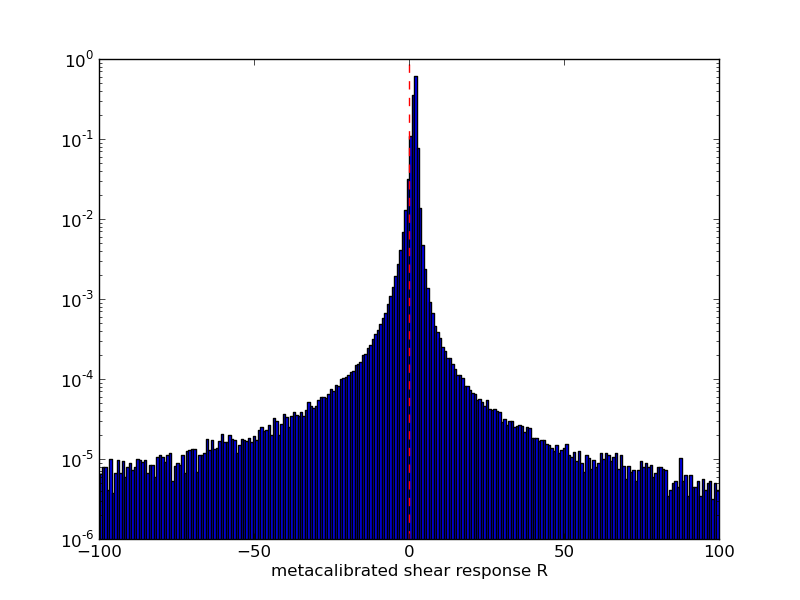
\includegraphics[width=0.45\textwidth]{./Plots/regauss-r-histogram.png}
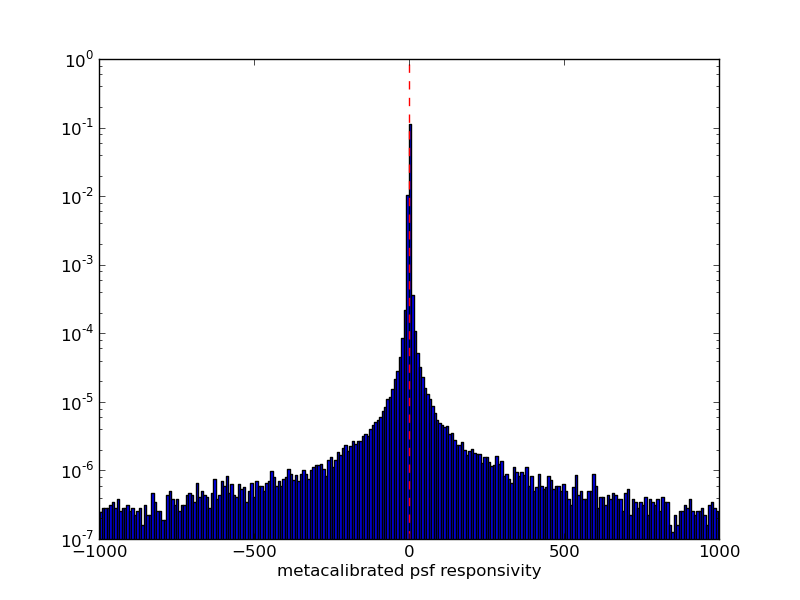
\includegraphics[width=0.45\textwidth]{./Plots/regauss-a-histogram.png}
\caption{{\bf Top:} Normalized distribution of meta-calibration shear responsivities from Regaussianization, on the Control-Ground-Constrant branch of the GREAT3 simulations.  {\bf Bottom:} Distribution of meta-calibration psf ellipticity responsivities from Regaussianization, on the Control-Ground-Constrant branch of the GREAT3 simulations. Vertical red dashed lines are drawn at zero for reference in both panels.}
\label{fig:calibhist}
\end{figure}


\begin{figure*}
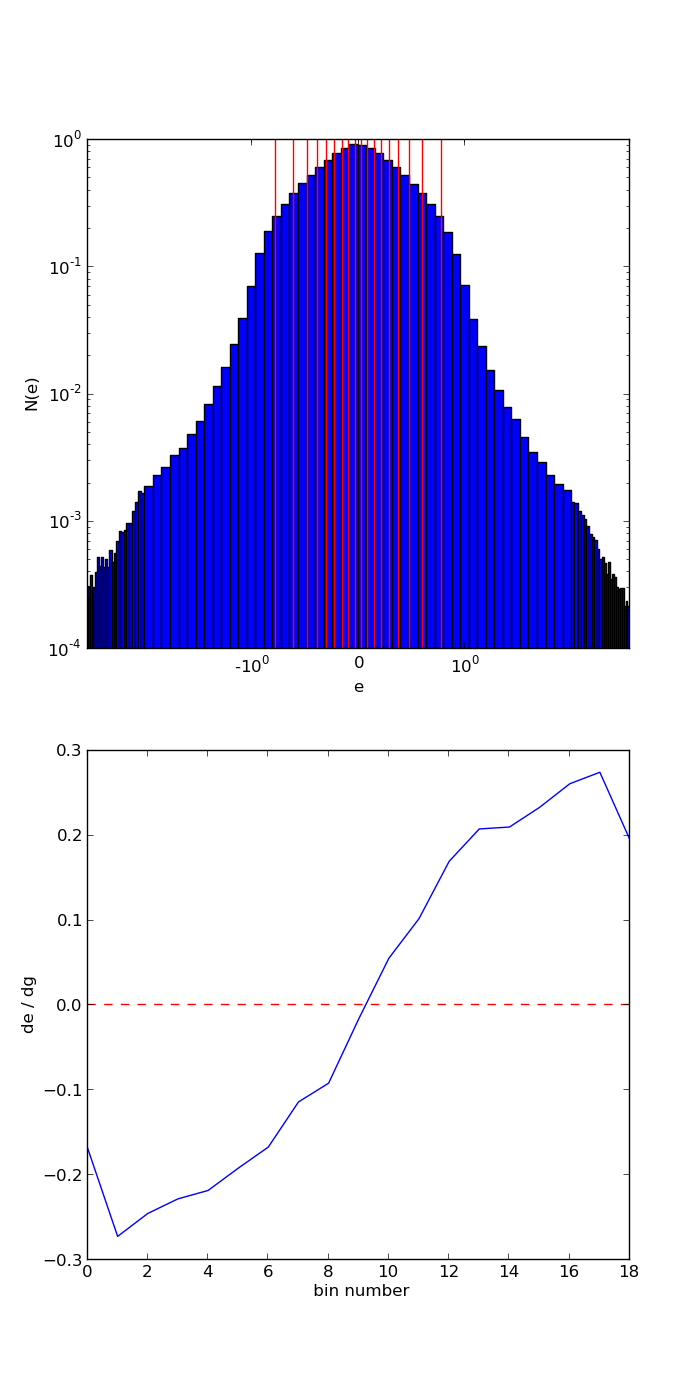
\includegraphics[width=0.3\textwidth]{./Plots/regauss-opt-shear_plots-prior_derivs.png}
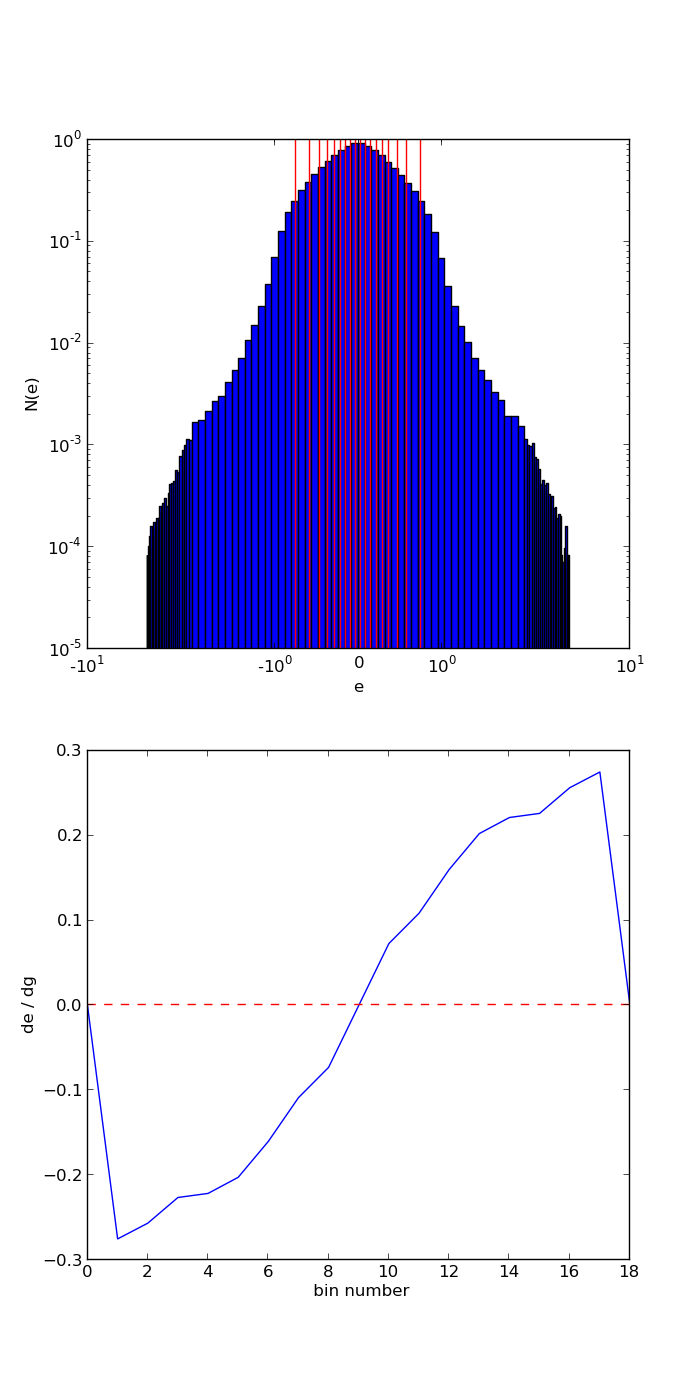
\includegraphics[width=0.3\textwidth]{./Plots/ksb-opt-shear_plots-prior_derivs.png}
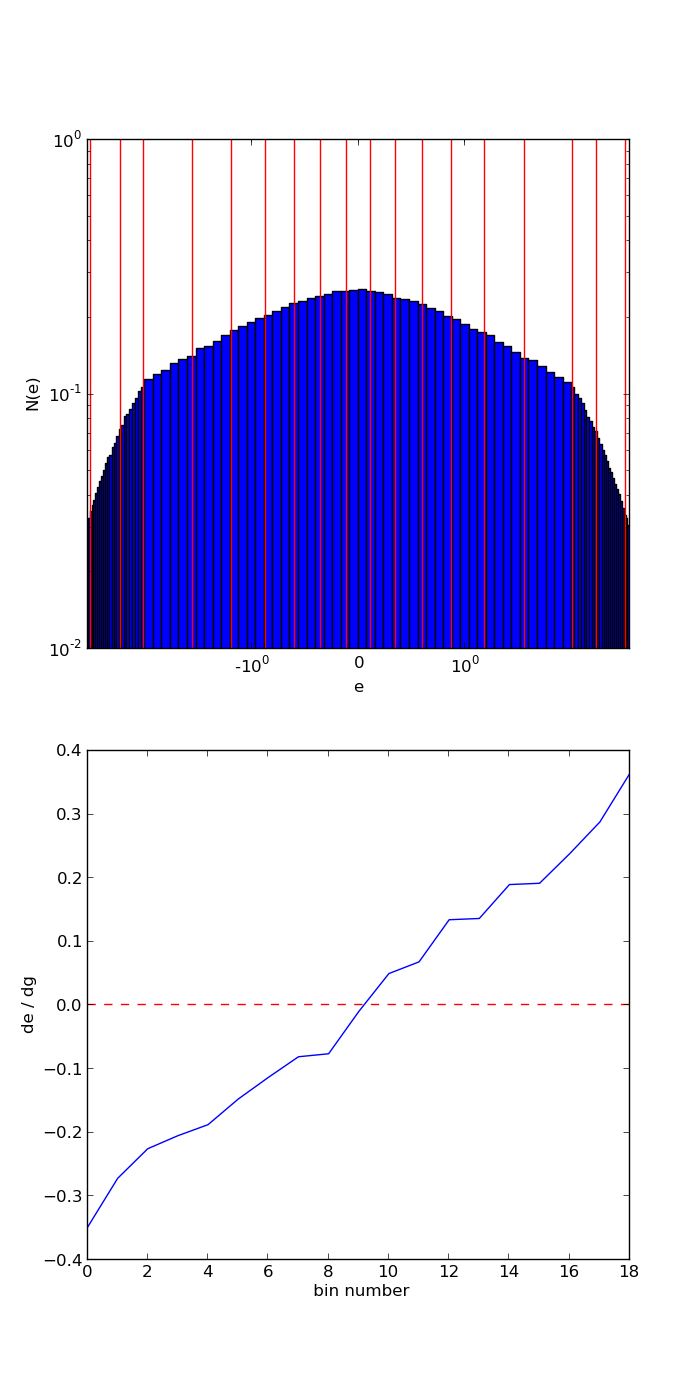
\includegraphics[width=0.3\textwidth]{./Plots/moments-opt-shear_plots-prior_derivs.png}
\caption{I do not like these figures. Treat them as placeholders for now.\\
Constructing the histogram estimator for the three shape measurement methods. {\bf Top} panels show measured shape distribution for each (from {\bf right} to {\bf left}) of the regauss, ksb, and moments methds. Vertical red lines show bin edges for a scheme with only 20 bins (much less than used in the estimation). {\bf Bottom} panels show the derivative $\frac{d\,p(e)}{d{e}}$ for each of the histograms. Abscissa are truncated at $\pm 4$, but the estimator runs over bins including all objects.
}
\label{fig:estimator}
\end{figure*}

If we have a poor model for the unlensed histogram, $h_{\rm fid}$, then the results will be biased. We can evaulate the distance from each field to the unlensed prior using equation~\ref{eqn:multnomial}, taking the probabilities $q_i$ from the unlensed prior and the histogram amplitudes from the current field, {after correcting for the estimated shear}. If the shear response measured for the unlensed prior is correct, then the performance of the estimator will depend only on the similarity of the prior to the measurement field. The likelihood can then be used as an objective criterion for the quality of the inference. 



\section{Testing Framework}
\towriterm{ brief-ish description of GREAT3 sims and sim framework. Basically, give enough info to show whats go- ing on and convince the reader that this is a non-trivially complicated dataset in terms of the PSFs and galaxy sam- ples. Also note difference from real life in terms of ex- pected mean shear, since thatll be important later.}


\subsection{Estimation Algorithms}
\towriterm{We picked three easily available estimation methods. Briefly describe each.}
\subsubsection{Regaussianization}
\towriterm{Brief description of regaussianization}
\subsubsection{KSB}
\towriterm{Brief description of KSB}
\subsubsection{Linear Moments}
\towriterm{Brief description of linear moments}


\subsection{Simulated Images}

\subsubsection{Control Ground Constant without Aberrations}
\towriterm{Brief description of this branch.}
\towriteemh{Performance expectations on this branch.}
\towriteemh{Briefly summarize calibration results for this branch.}
\todorm{One of us should obtain ksb metacalibration catalogs for this branch. Rachel can give Eric the images, or generate the MC catalogs herself, whichever works.}
\todorm{One of us should obtain moments metacalibration catalogs for this branch. Rachel can give Eric the images, or generate the MC catalogs herself, whichever works.}


\subsubsection{Real Ground Constant without Aberrations}

The first branch we analyze is the simplest. The galaxy models Sersic profiles, and the realization of galaxy parameters is that of the CGC branch of GREAT3. We have generated new images with simpler psf models, keeping the atmospheric component but removing the optical aberrations. 
\towriterm{Brief description of this branch.}
\towriteemh{Performance expectations on this branch.}
\towriteemh{Briefly summarize calibration results for this branch.}
\todorm{One of us should obtain ksb metacalibration catalogs for this branch. Rachel can give Eric the images, or generate the MC catalogs herself, whichever works.}
\todorm{One of us should obtain moments metacalibration catalogs for this branch. Rachel can give Eric the images, or generate the MC catalogs herself, whichever works.}



\subsubsection{Control Ground Constant with Aberrations}
\towriterm{Brief description of this branch.}
\towriteemh{Performance expectations on this branch.}
\towriteemh{Briefly summarize calibration results for this branch.}

\subsubsection{Real Ground Constant with Aberrations}
\towriterm{Brief description of this branch.}
\towriteemh{Performance expectations on this branch.}
\towriteemh{Briefly summarize calibration results for this branch.}
\todoemh{Generate ksb metacalibration catalogs for this branch. }
\todoemh{Generate moments metacalibration catalogs for this branch.}
\toplotemh{Plot ksb results for this branch.}
\toplotemh{Plot moment results for this branch.}

\subsubsection{Control or Real Ground Constant with constant Aberrations}
\towriterm{Brief description of this branch.}
\towriteemh{Performance expectations on this branch.}
\towriteemh{Briefly summarize calibration results for this branch.}
\todorm{Generate images and catalogs for this branch.}
\toplotemh{Plot regauss results for this branch.}
\toplotemh{Plot ksb results for this branch.}
\toplotemh{Plot moment results for this branch.}





\begin{figure*}
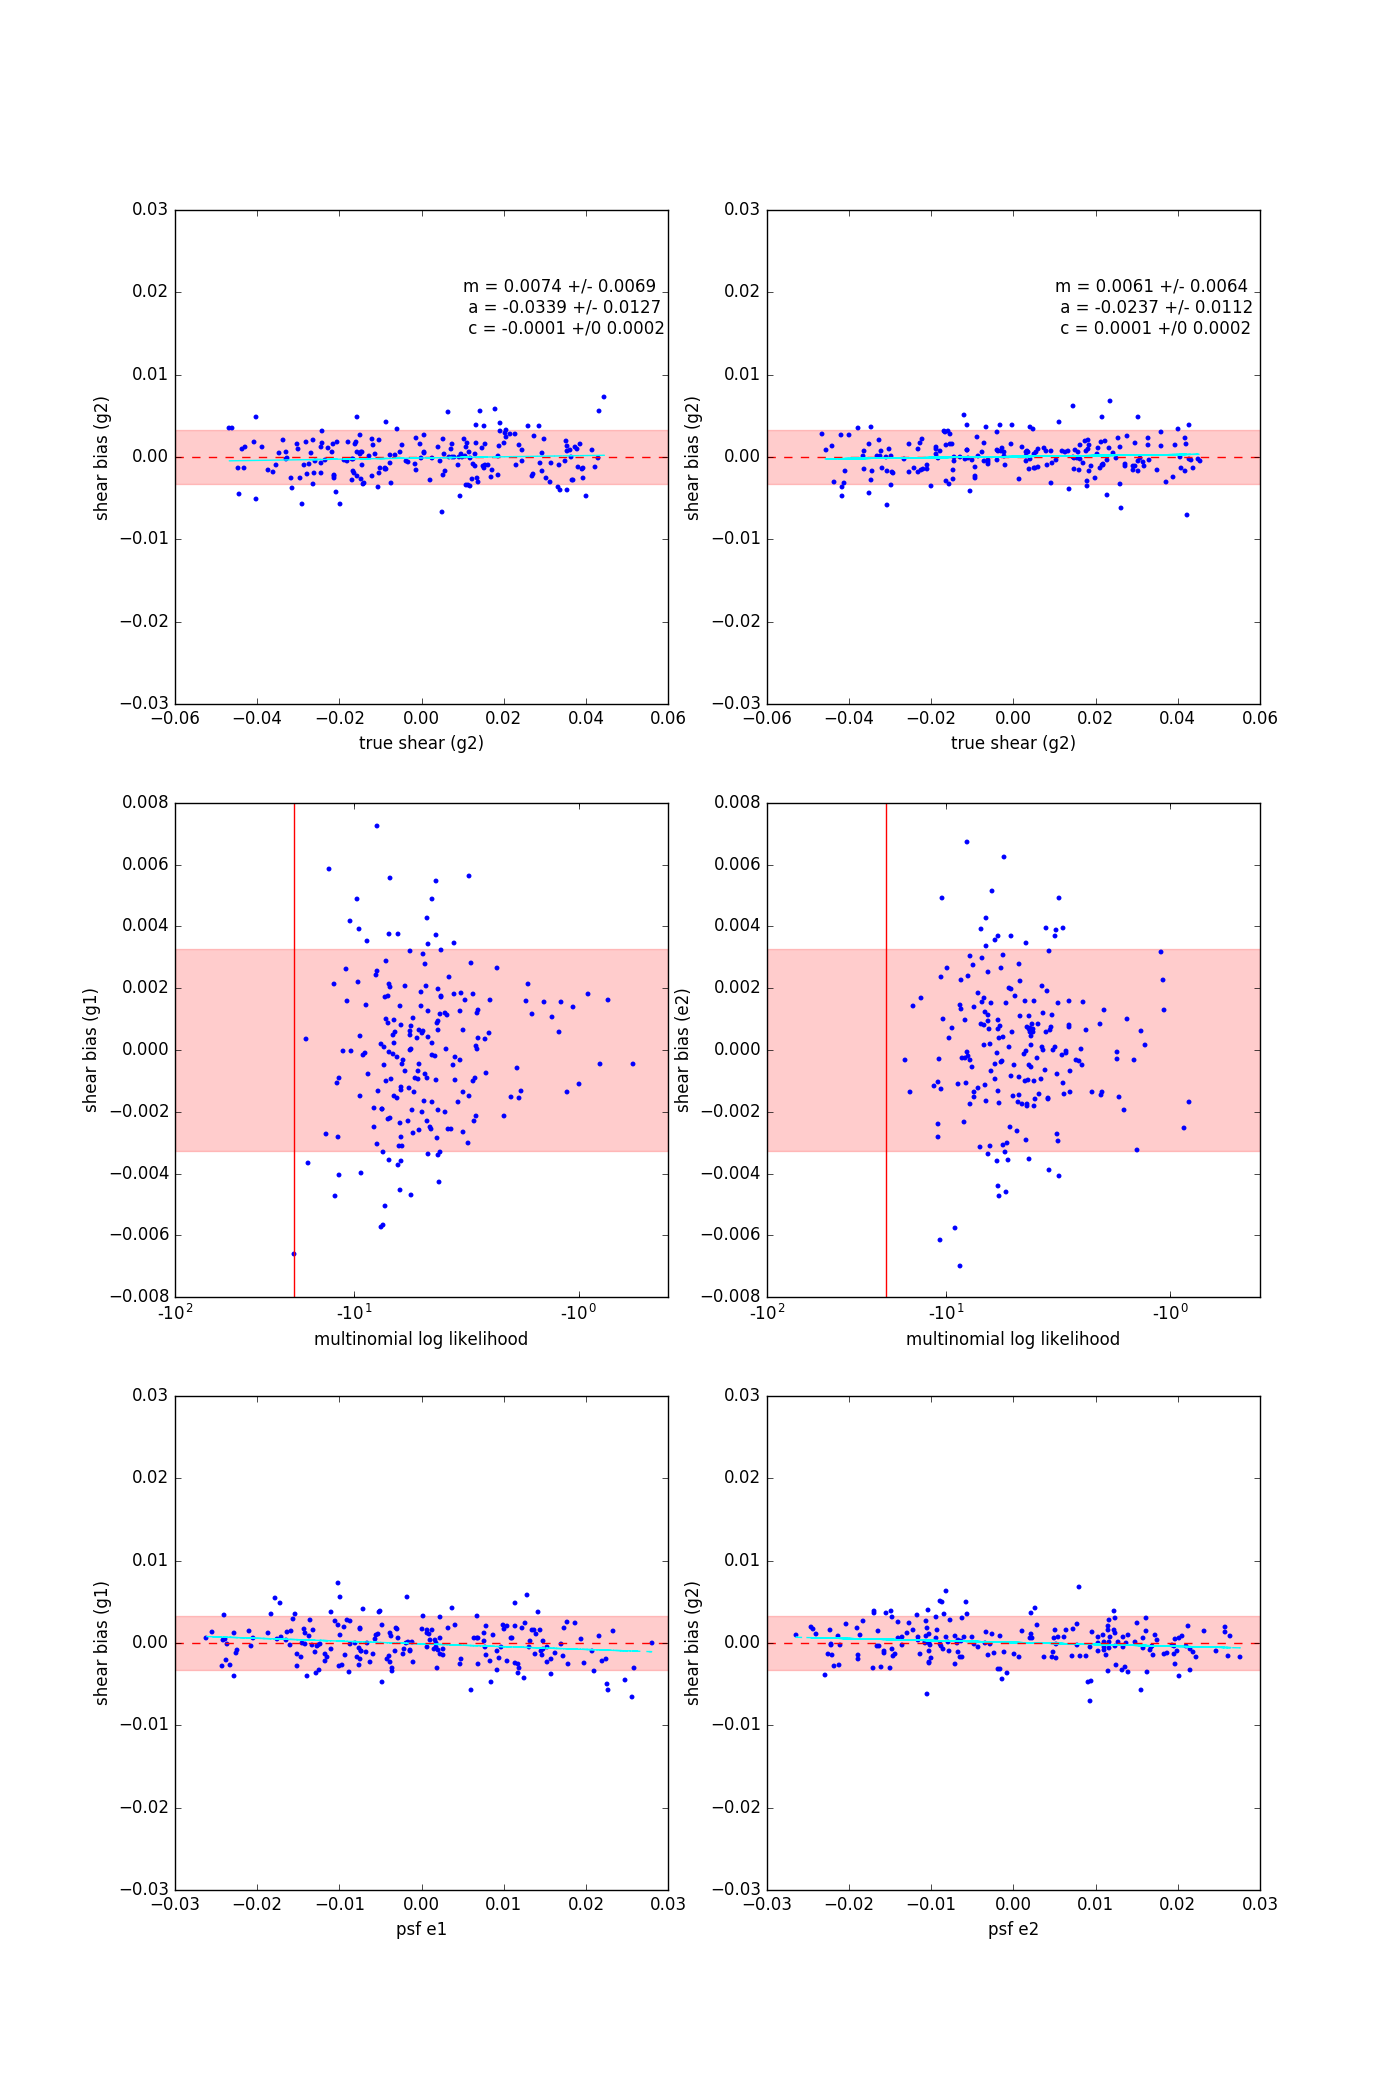
\includegraphics[width=0.31\linewidth]{./Plots/noaber-regauss-opt-shear_plots.png}
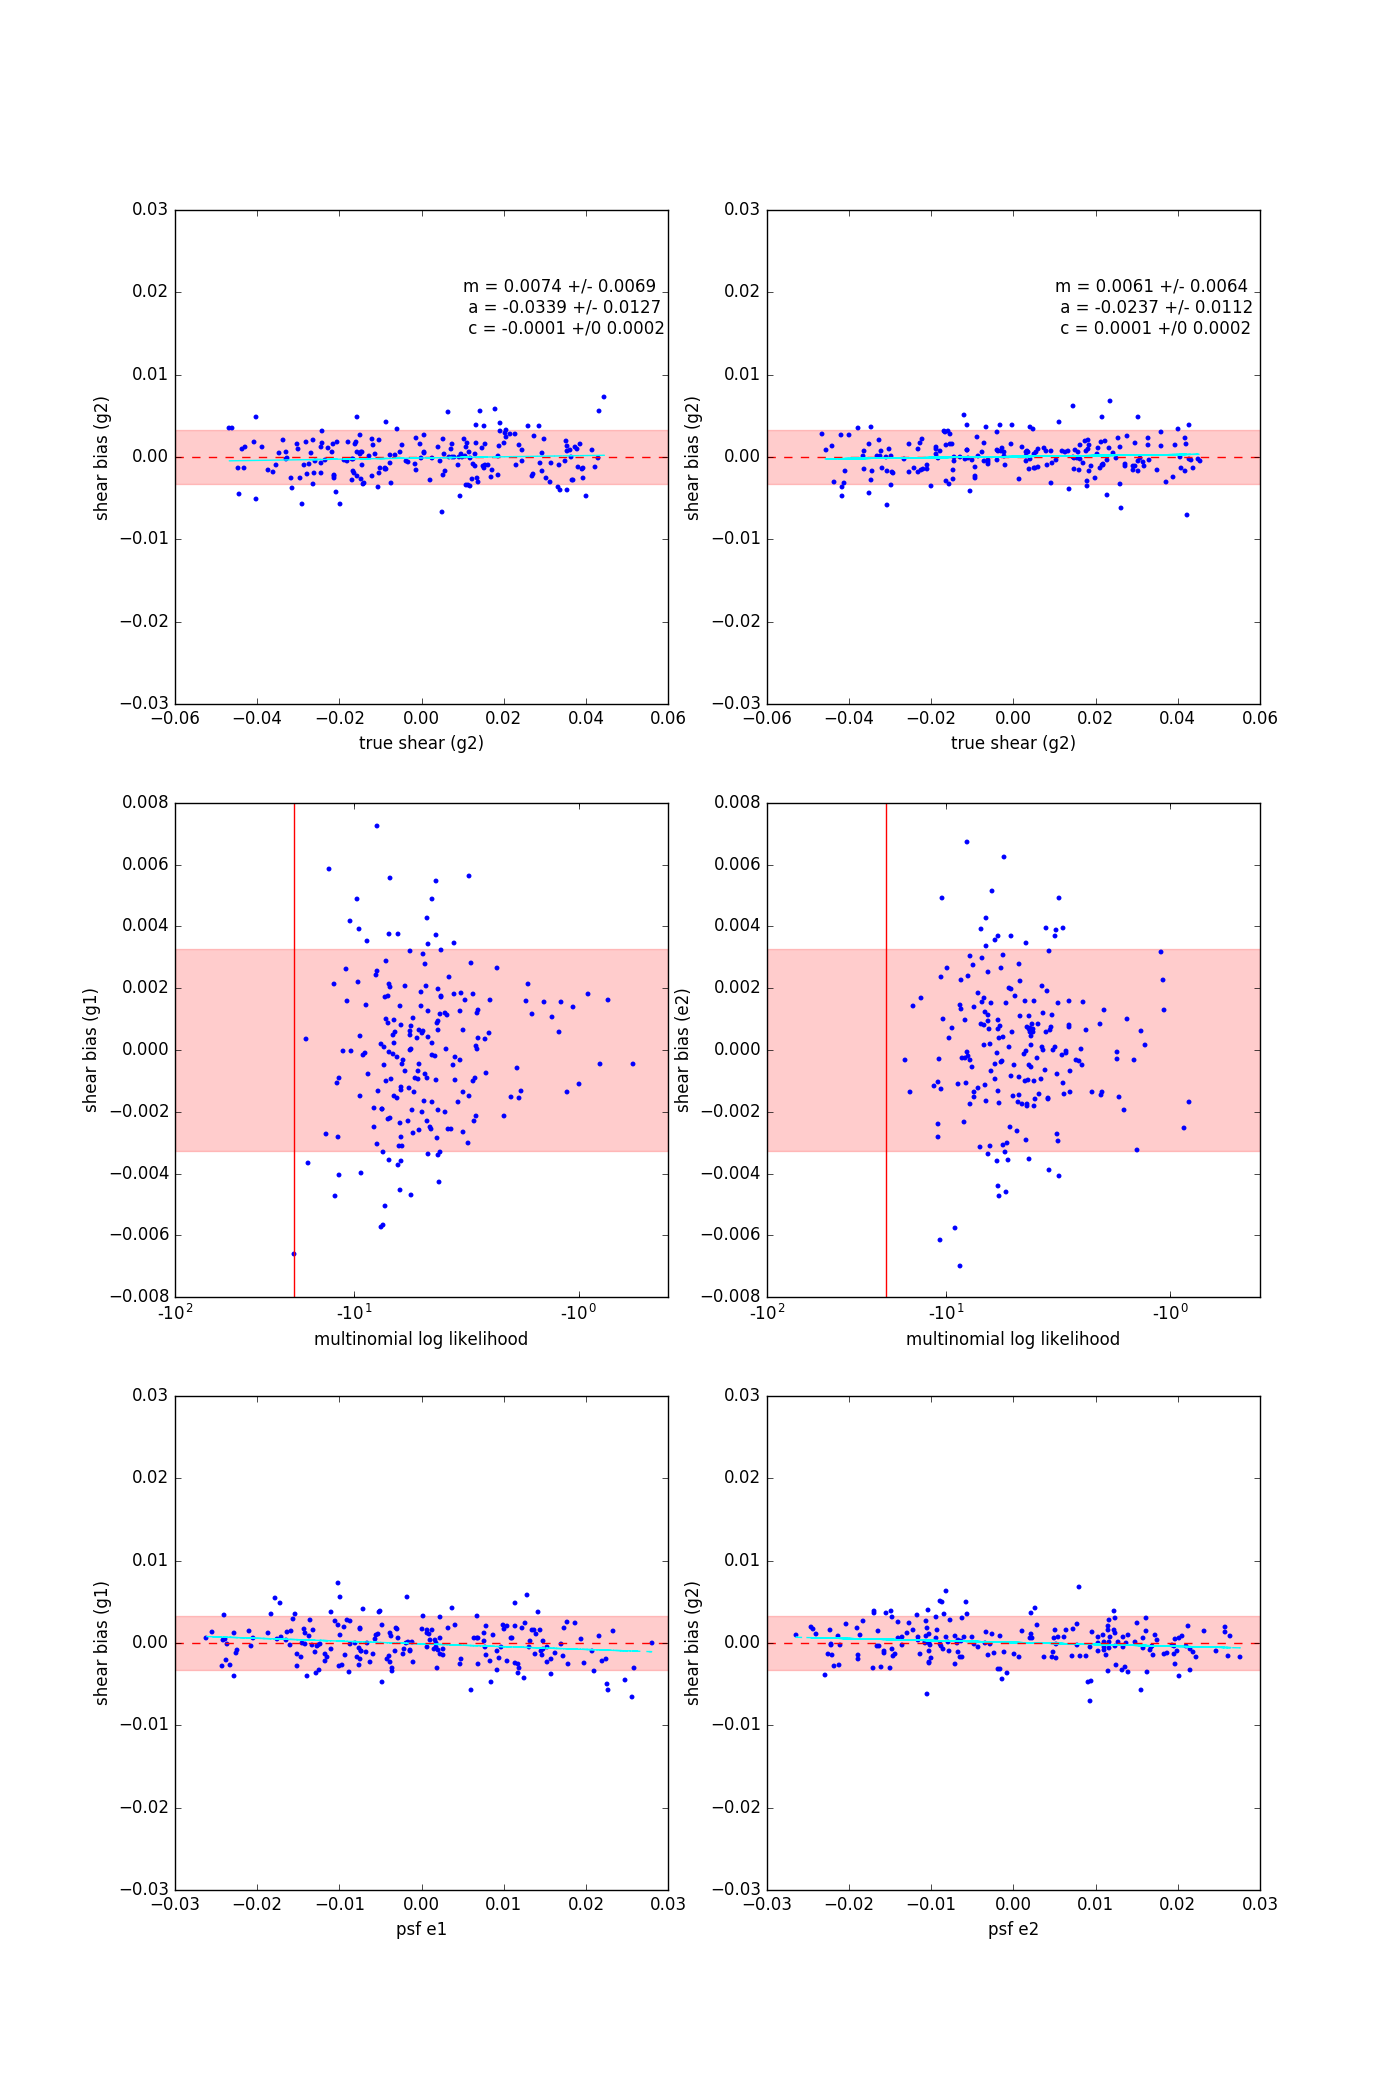
\includegraphics[width=0.31\linewidth]{./Plots/noaber-regauss-opt-shear_plots.png}
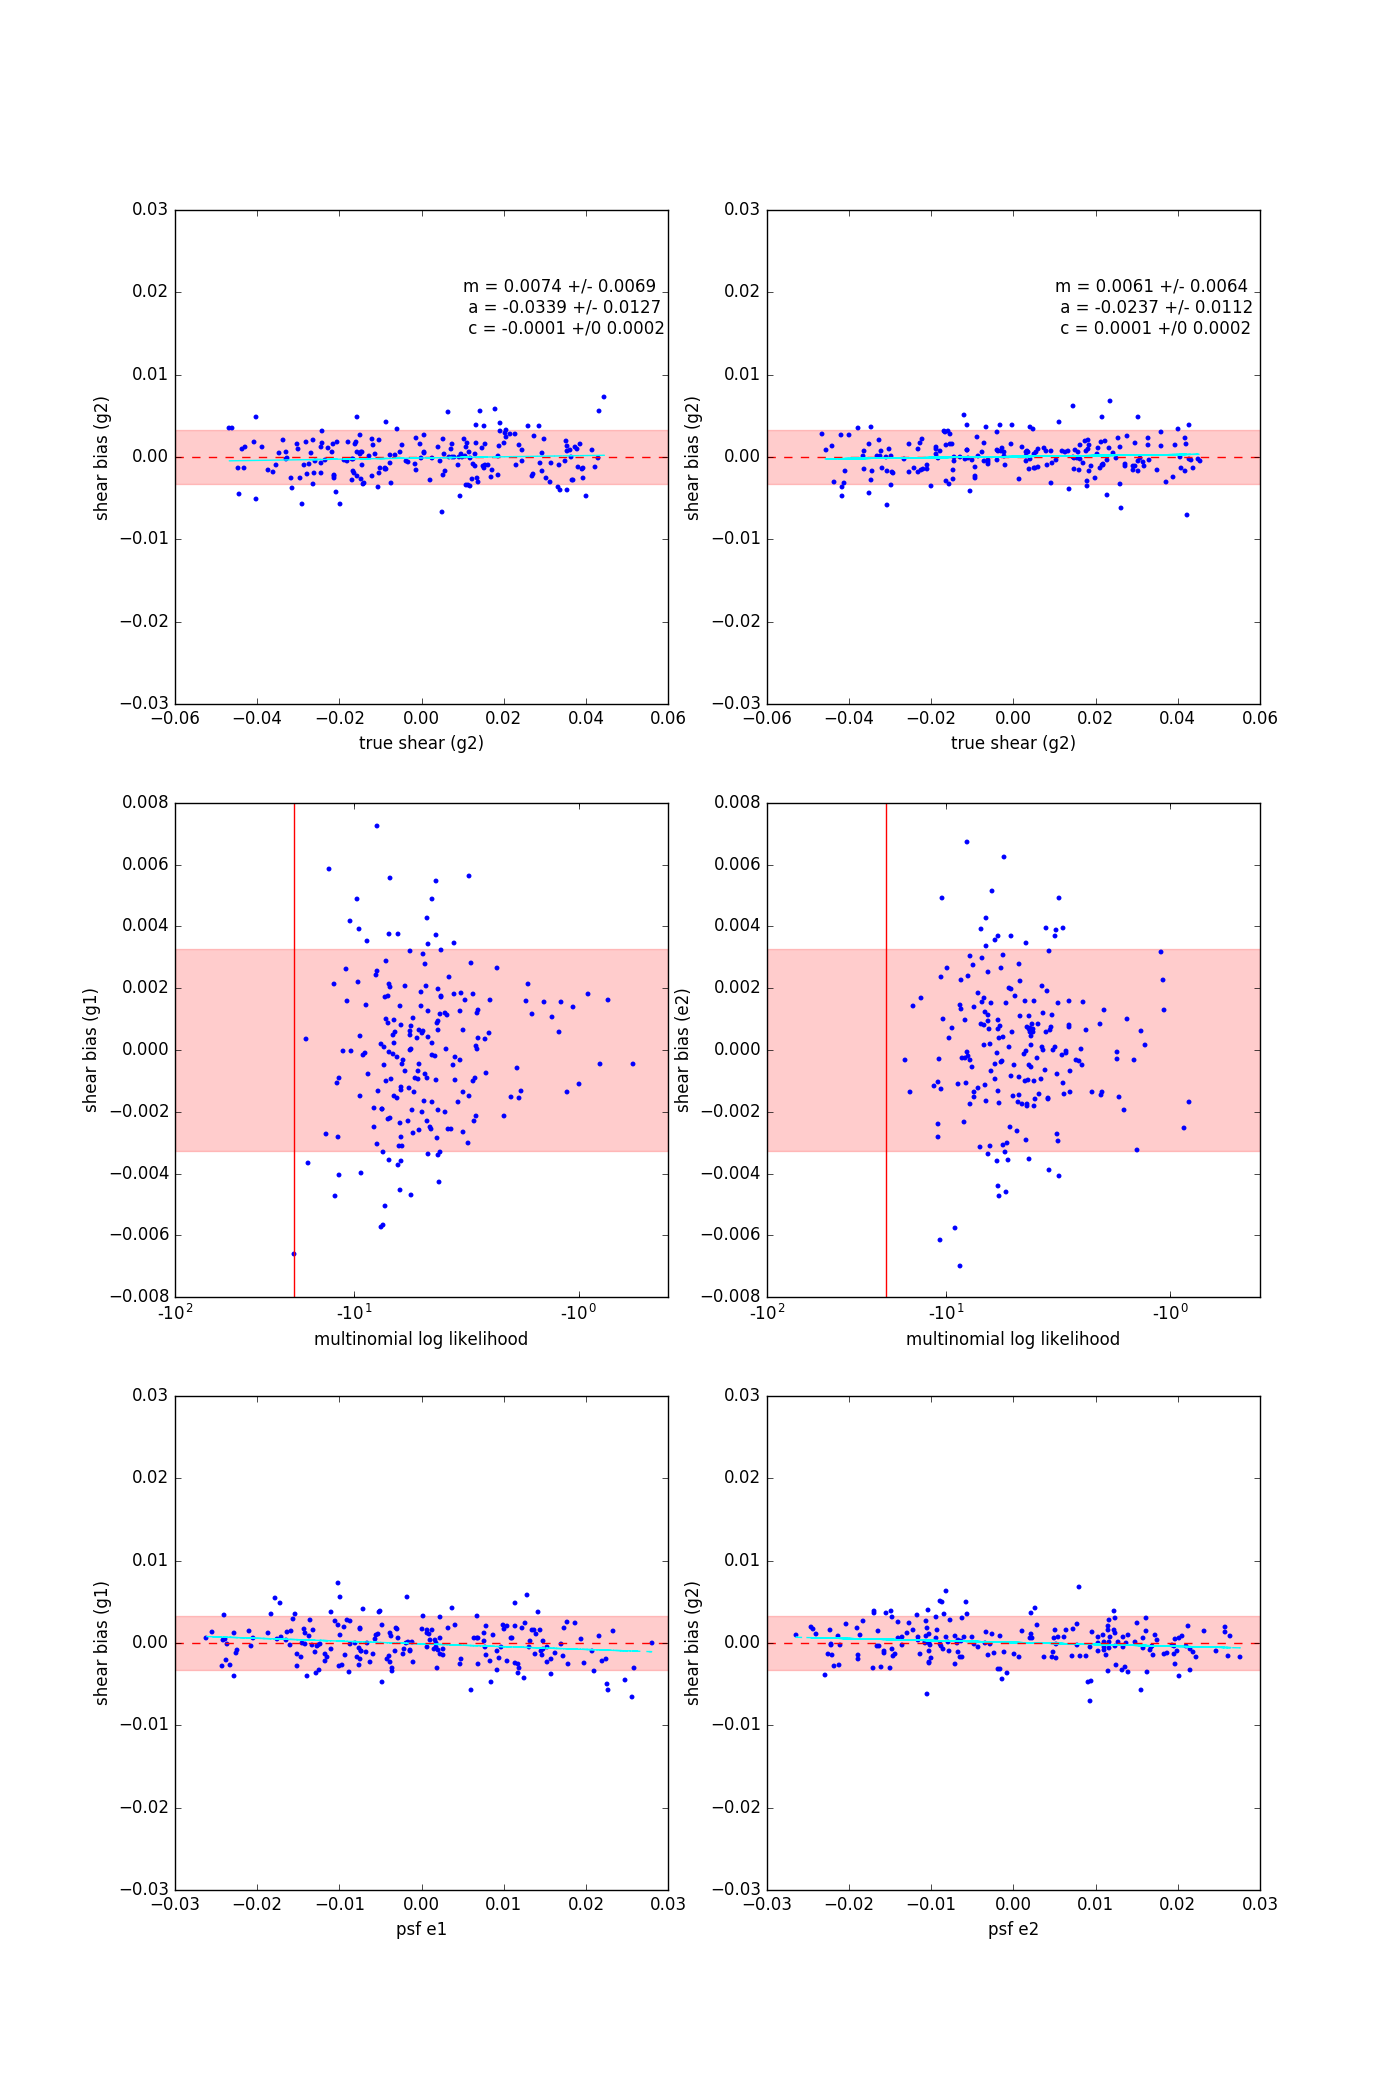
\includegraphics[width=0.31\linewidth]{./Plots/noaber-regauss-opt-shear_plots.png}
\caption{Results of metacalibration for regauss on CGC-no aberrations}
\end{figure*}


\begin{figure*}
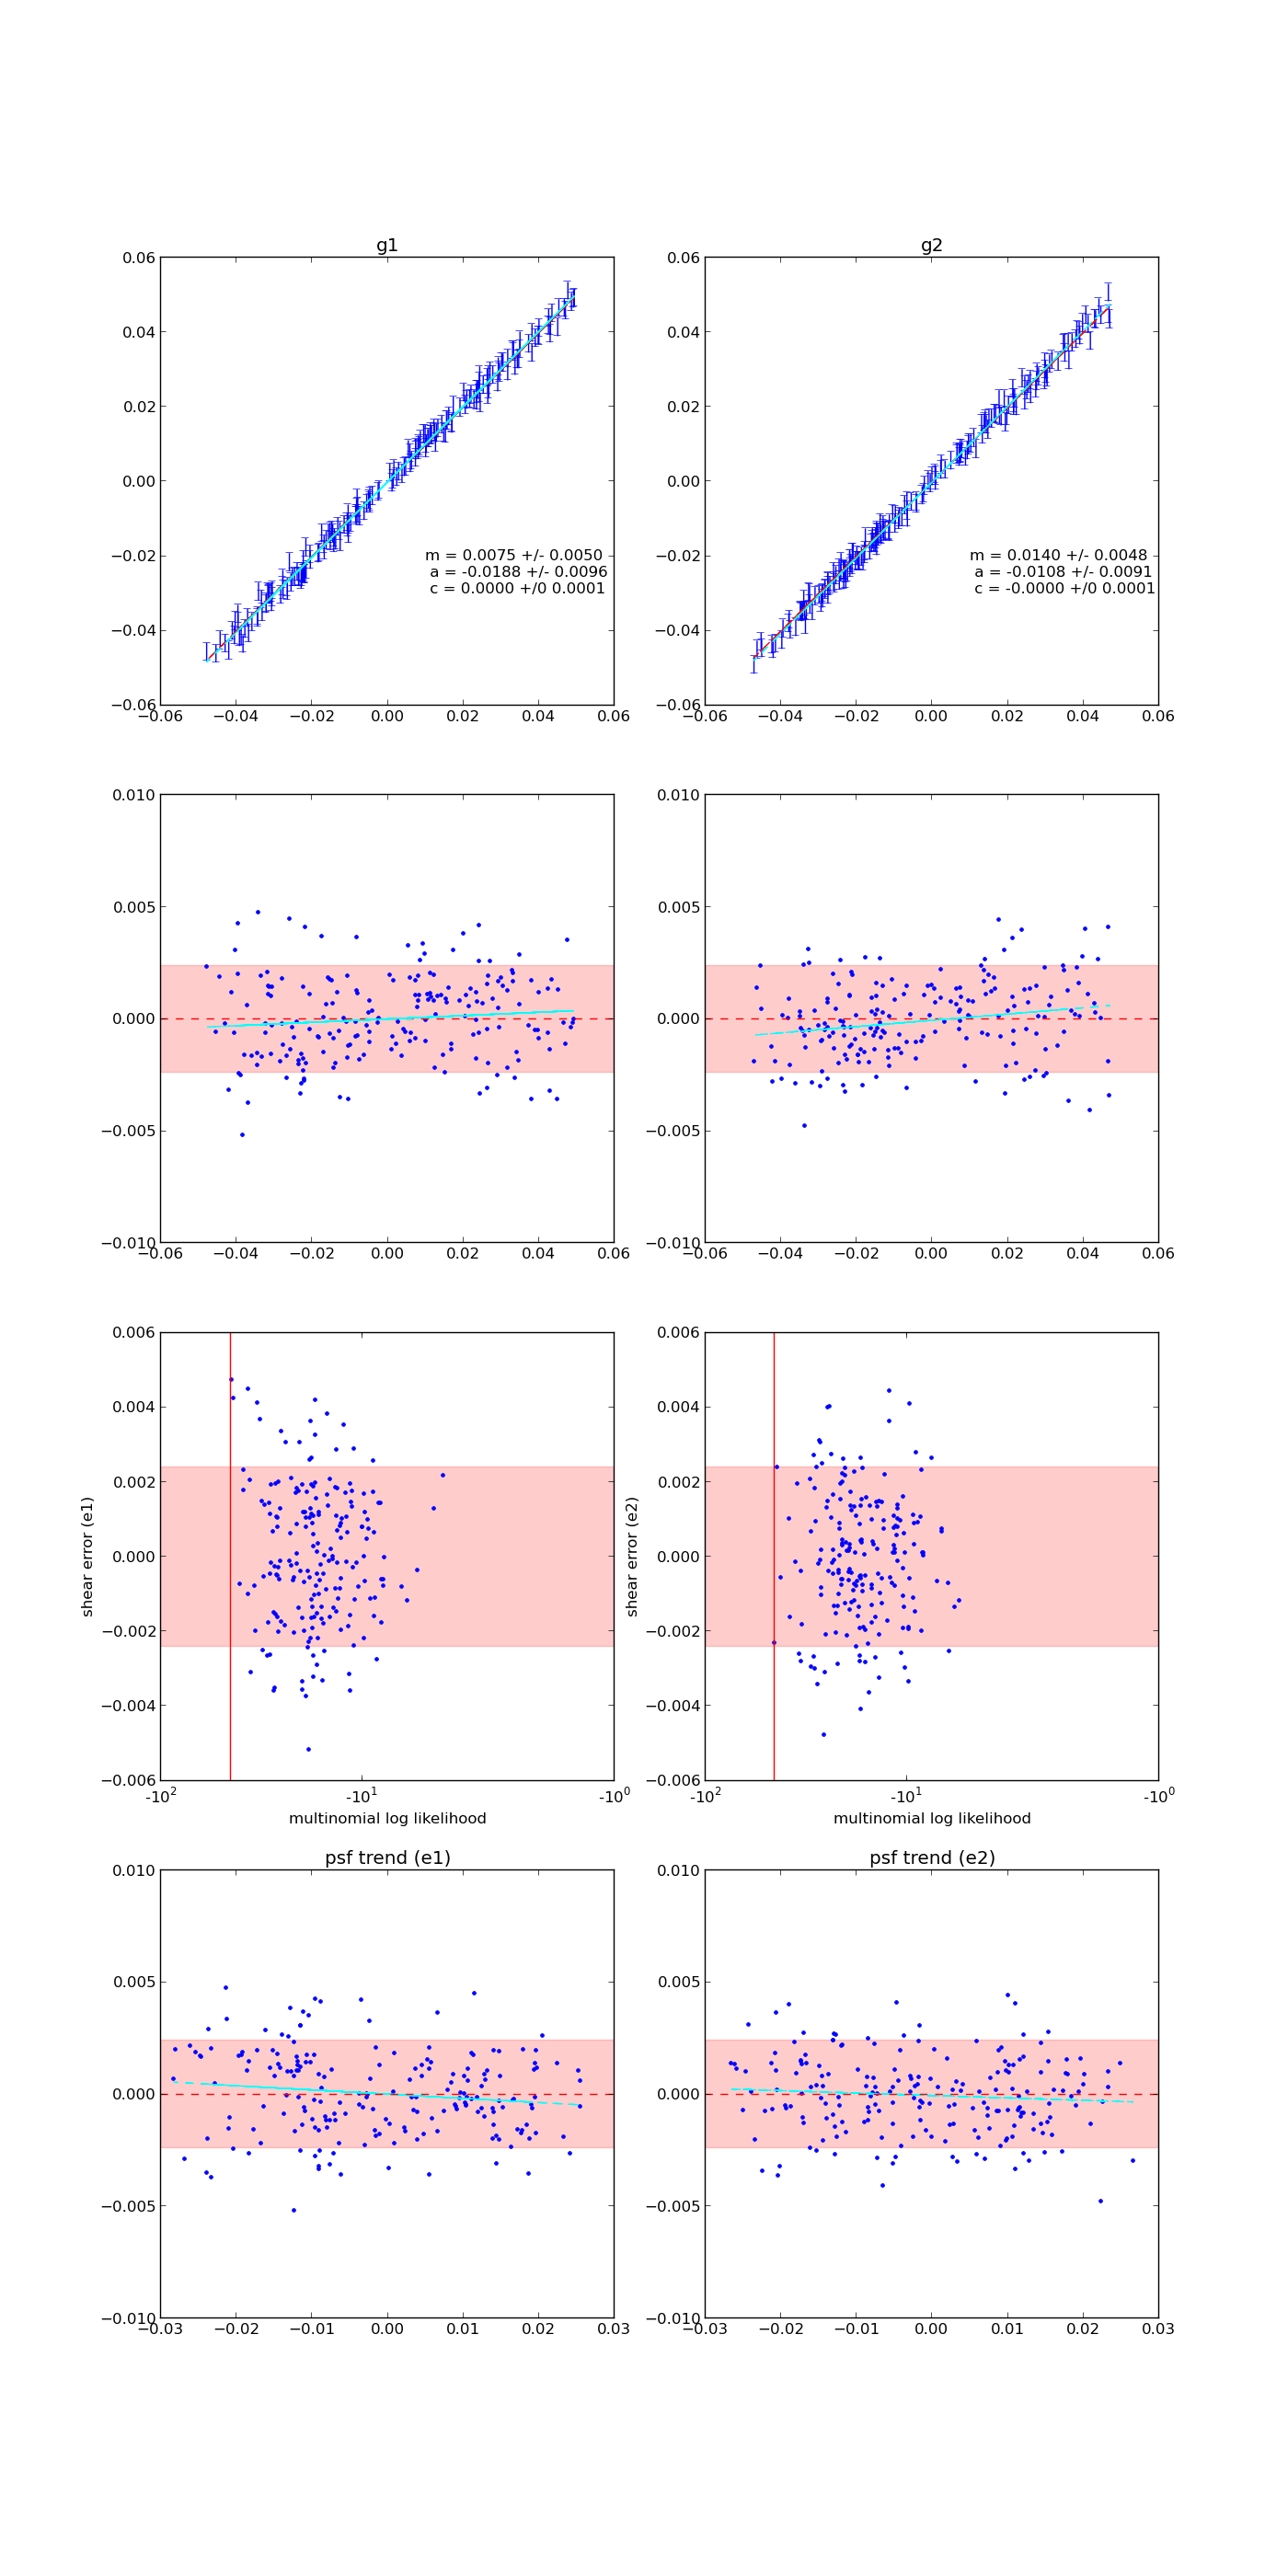
\includegraphics[width=0.31\linewidth]{./Plots/rgc-noaber-regauss-opt-shear_plots.png}
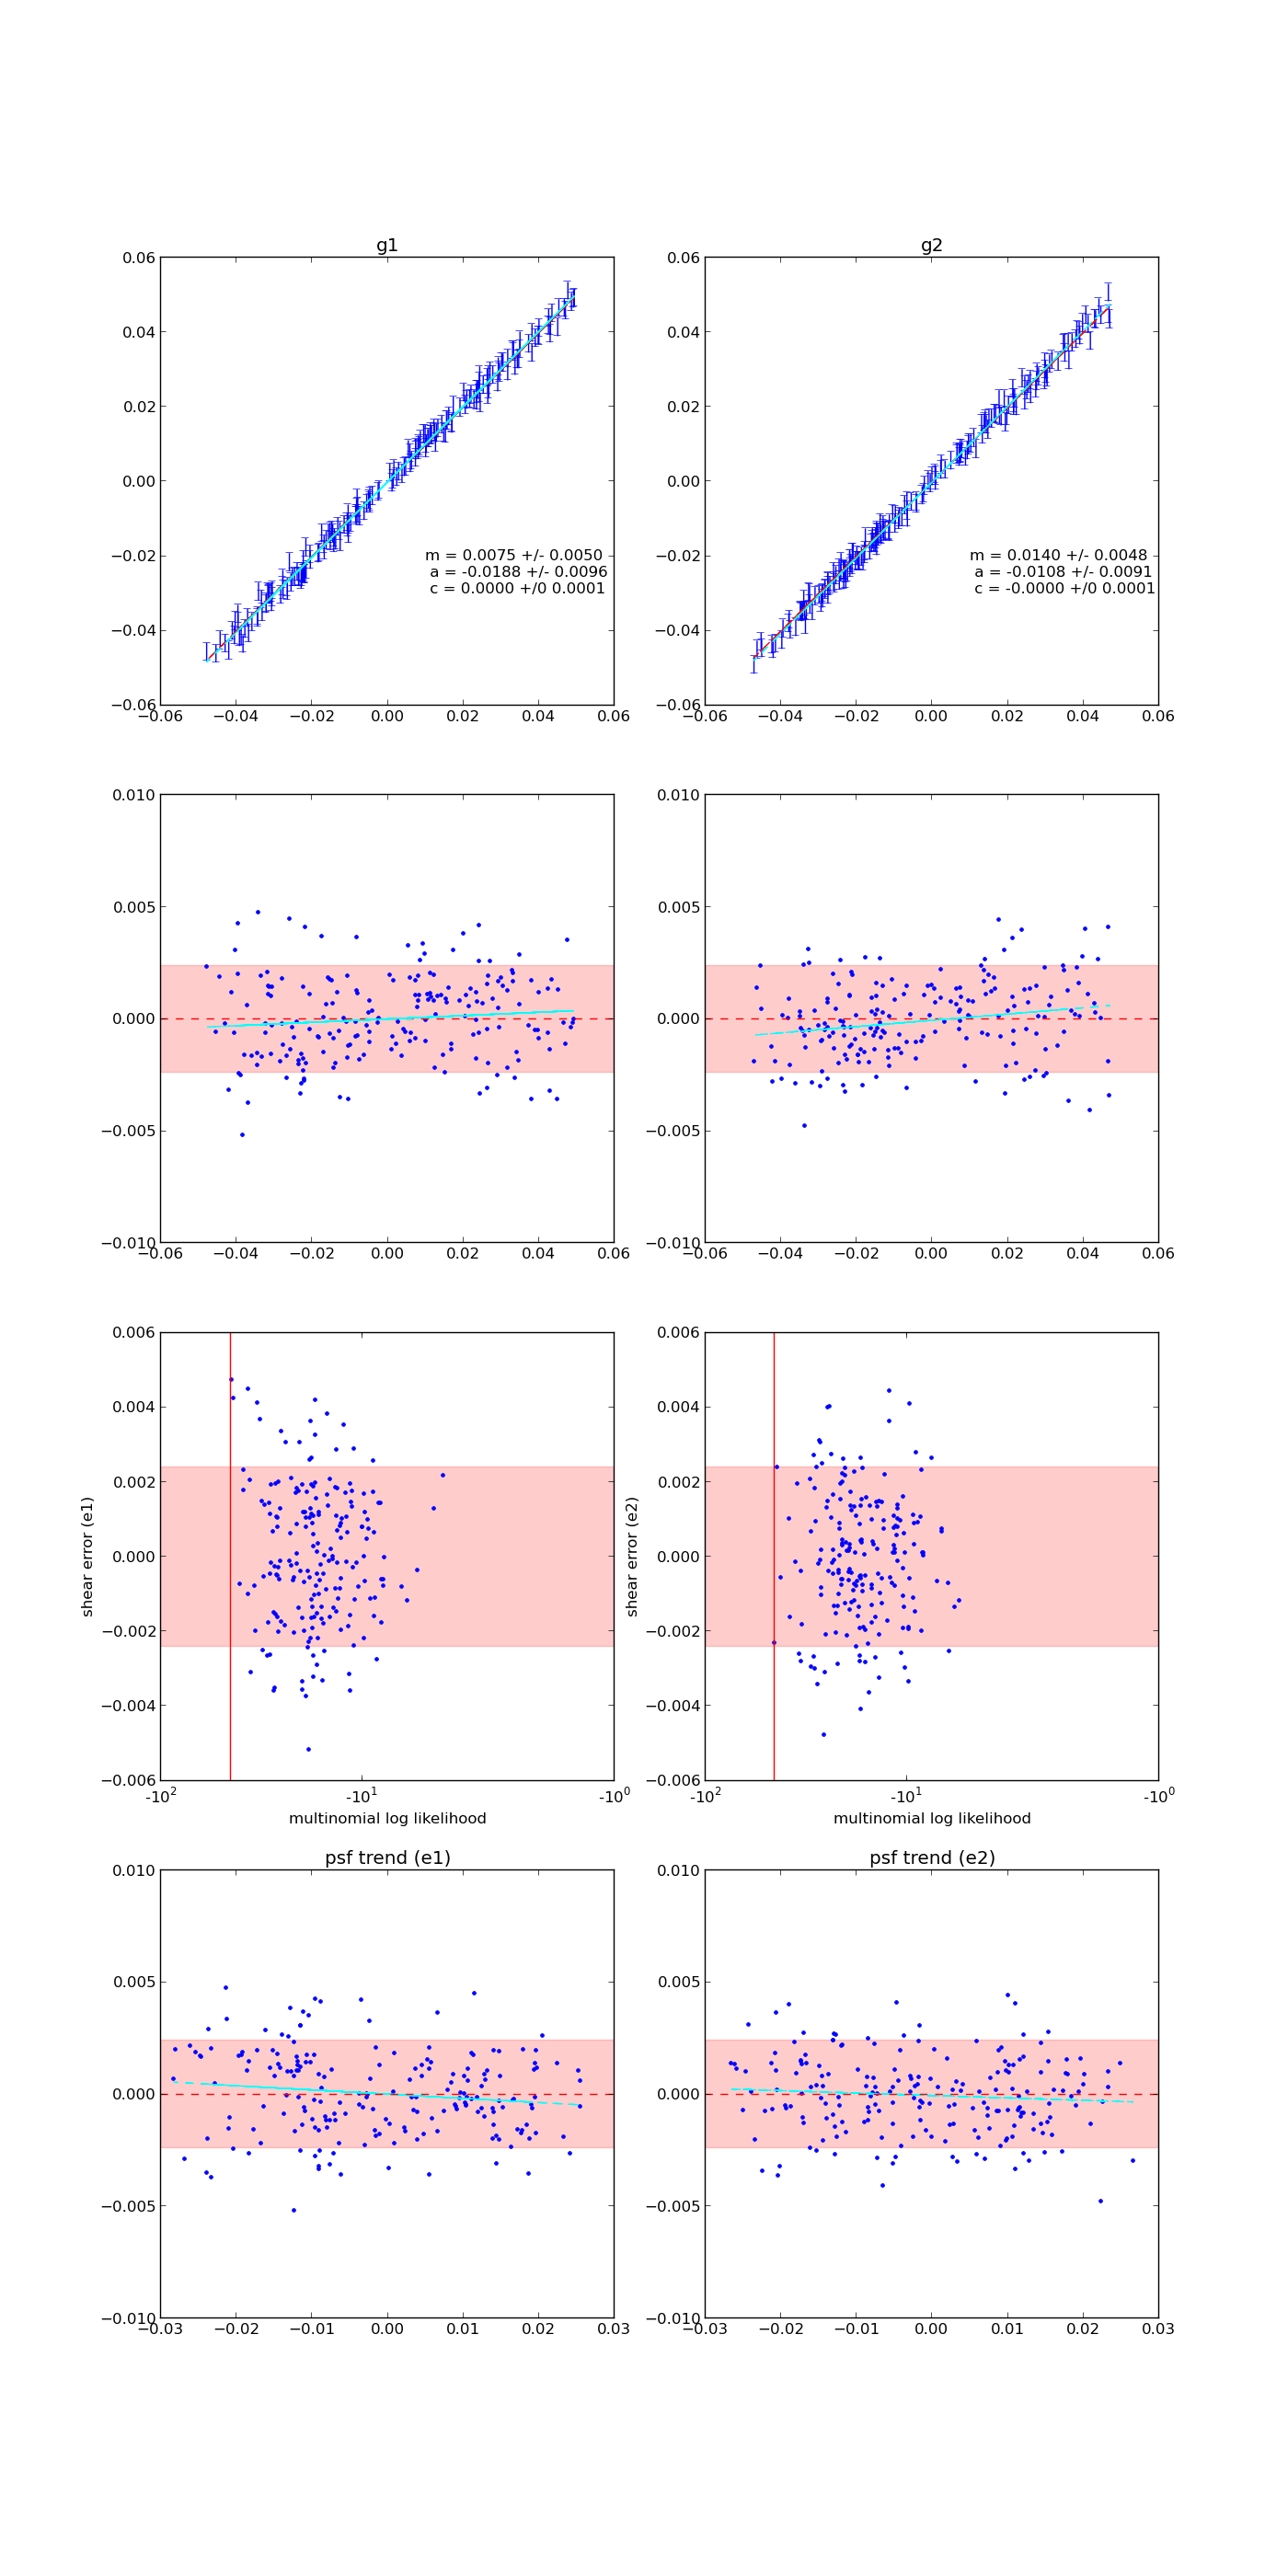
\includegraphics[width=0.31\linewidth]{./Plots/rgc-noaber-regauss-opt-shear_plots.png}
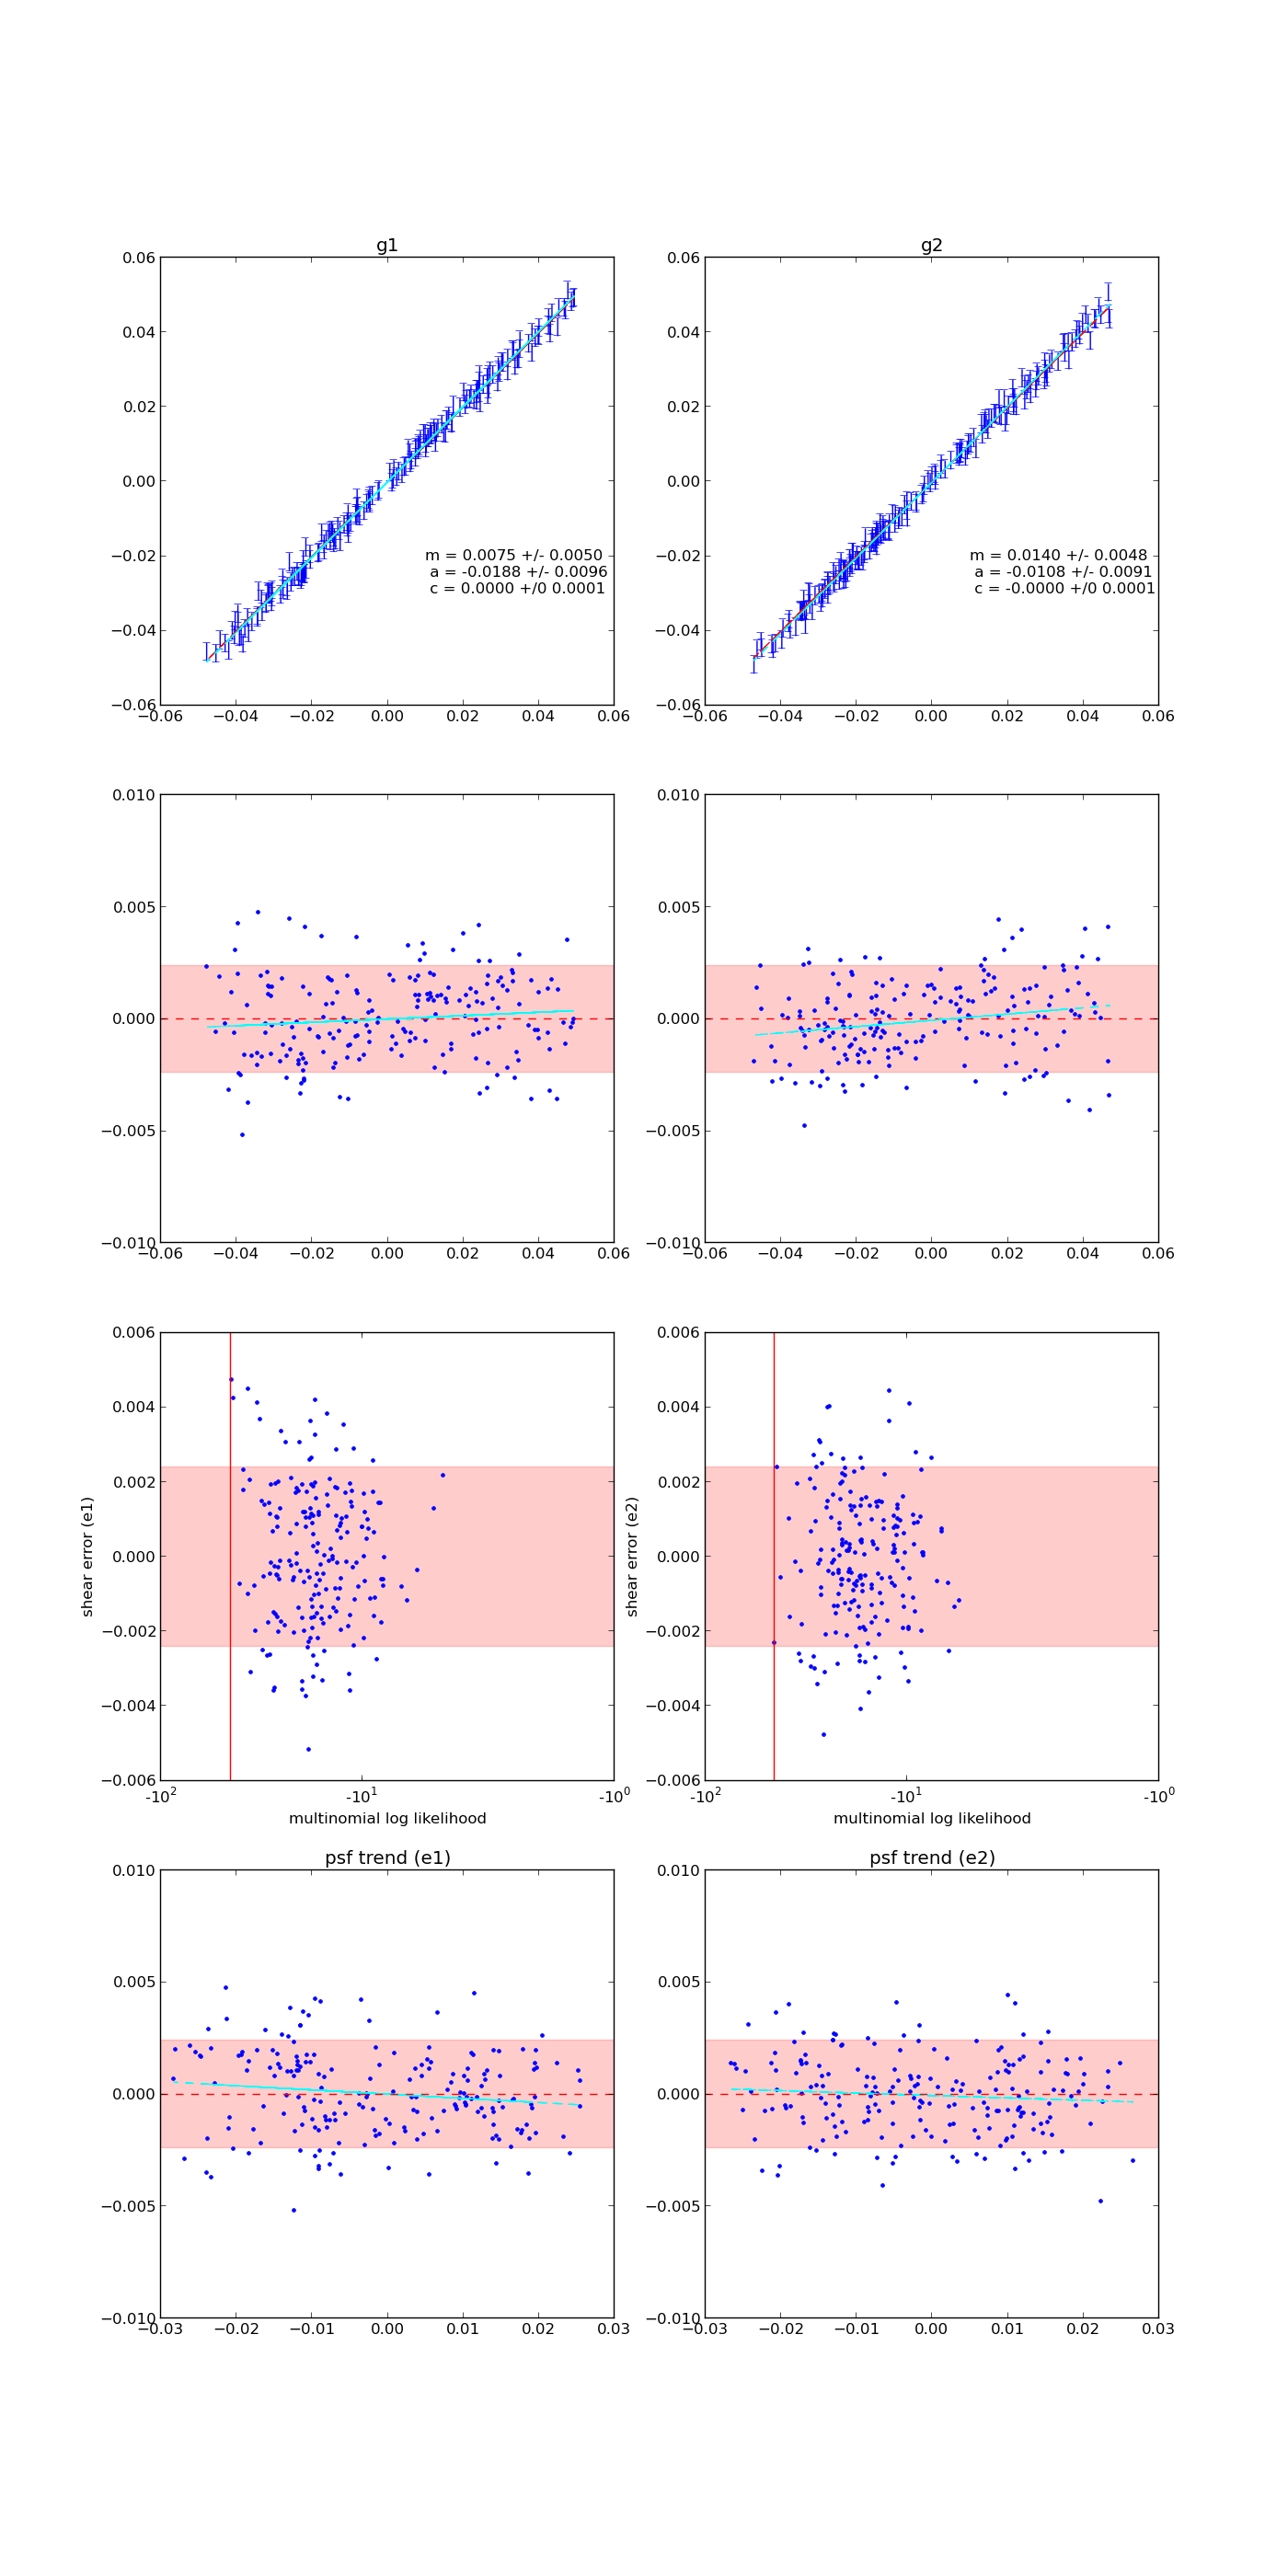
\includegraphics[width=0.31\linewidth]{./Plots/rgc-noaber-regauss-opt-shear_plots.png}
\caption{Results of metacalibration for regauss on CGC with no aberrations. From {\bf right} to {\bf left}: regauss, ksb, moments. Note that we do not have these results for ksb and moments yet.}
\end{figure*}

\begin{figure*}
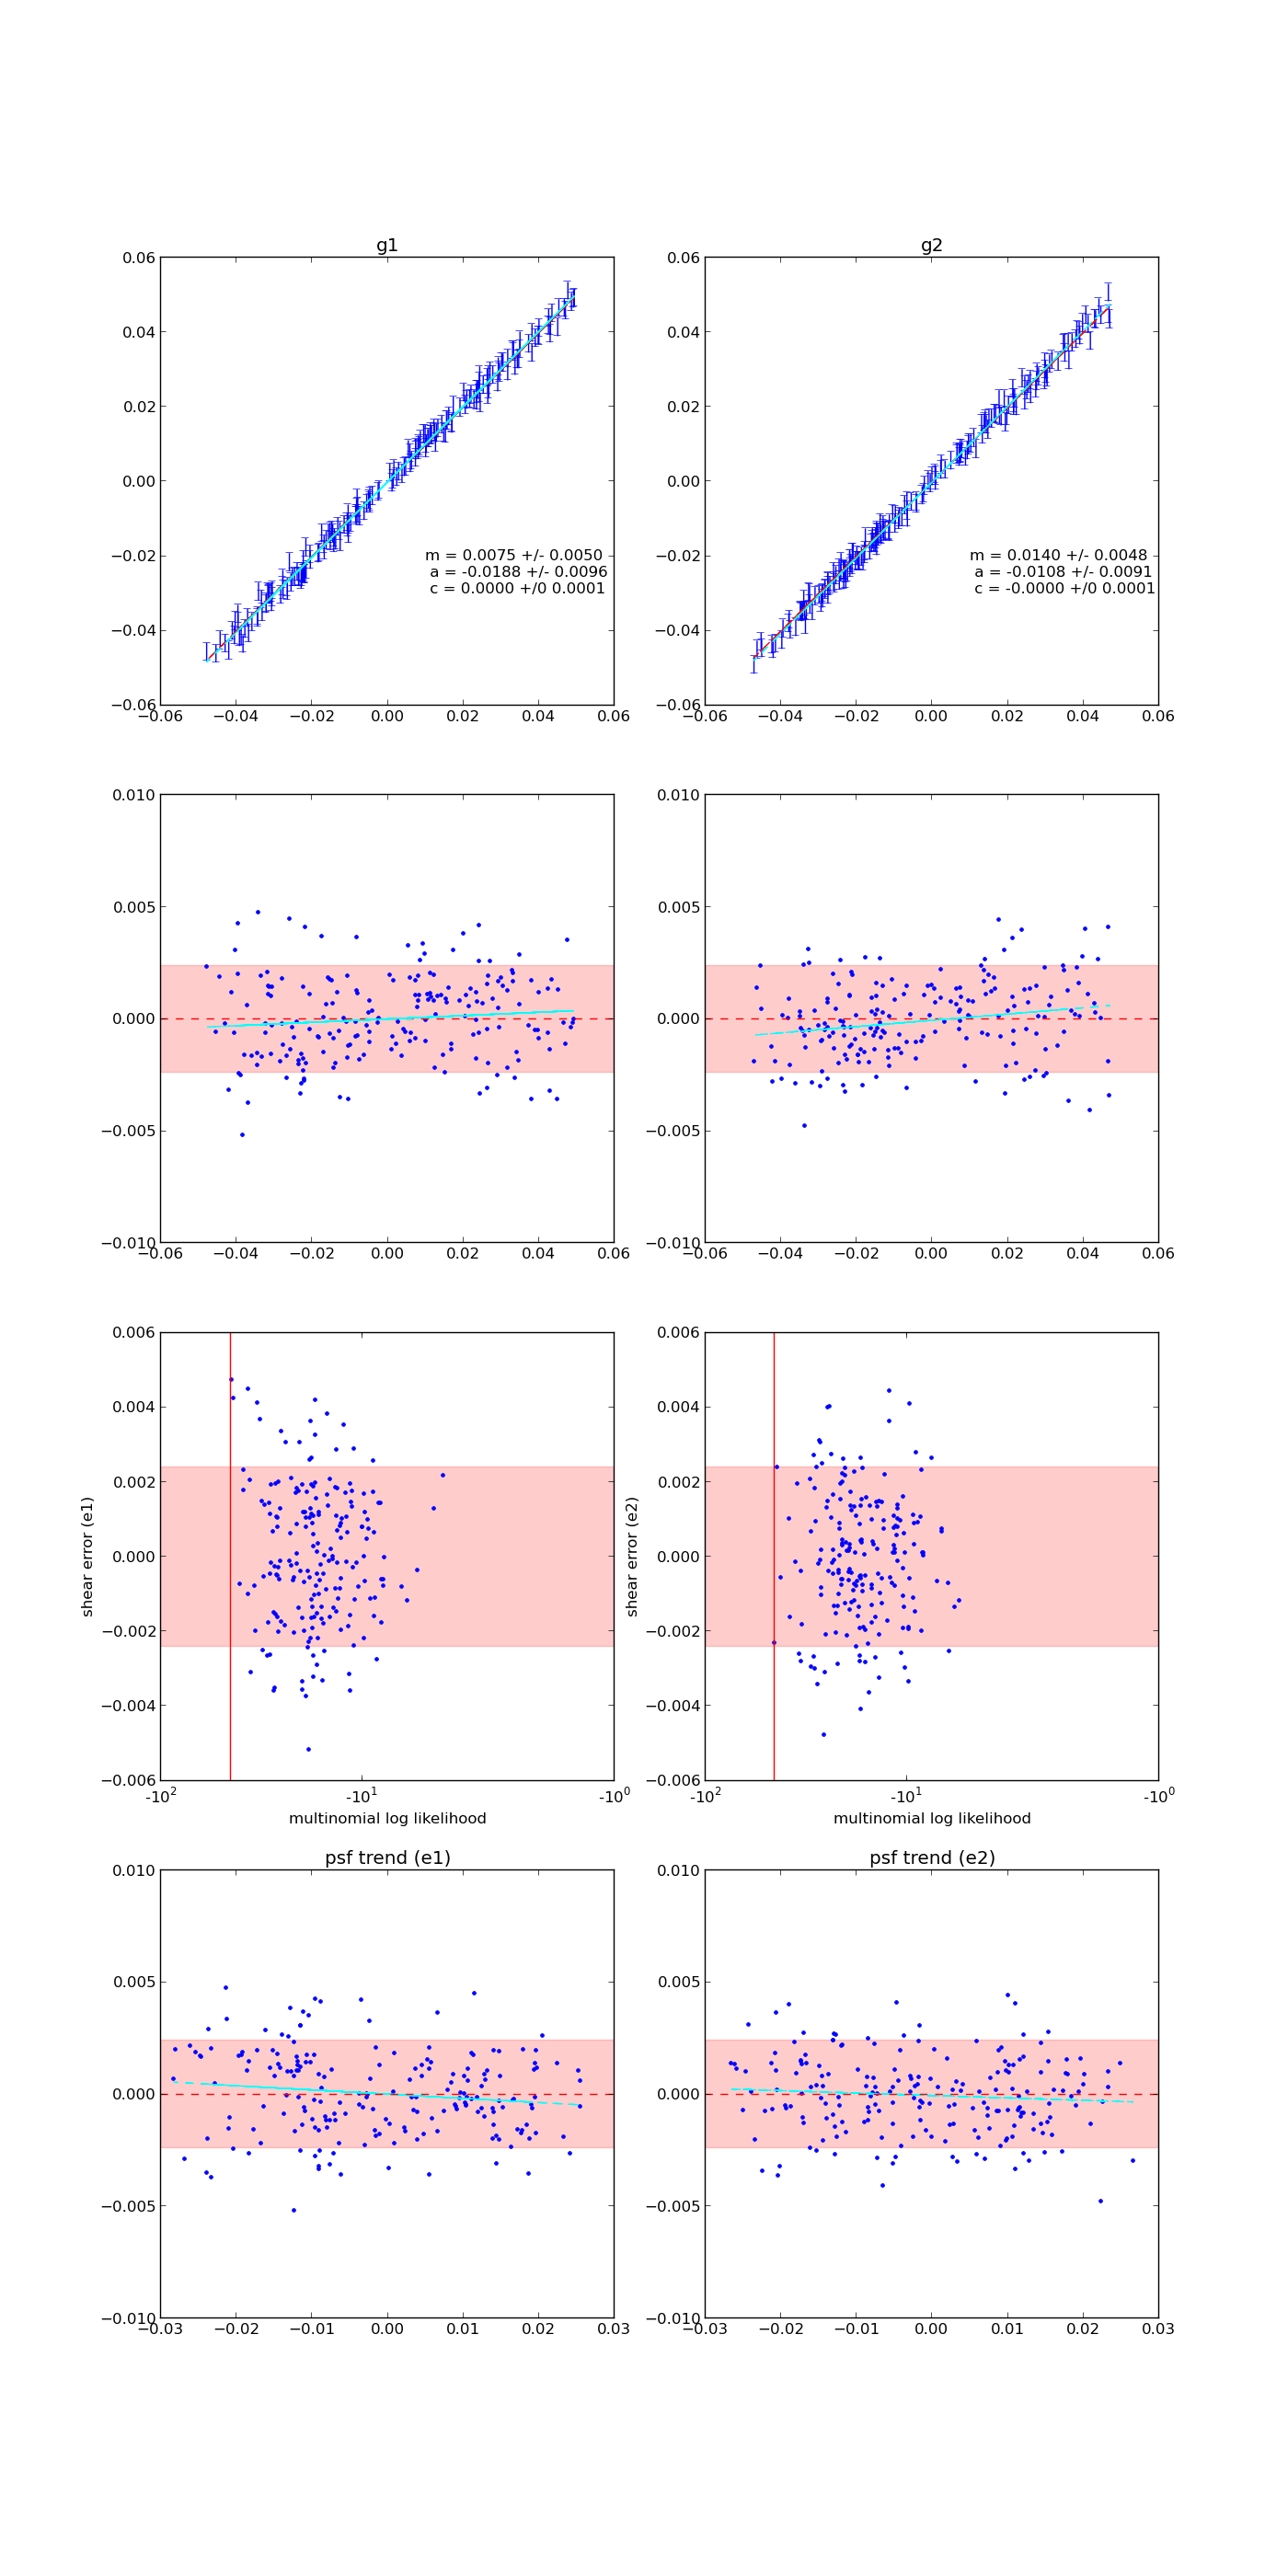
\includegraphics[width=0.31\linewidth]{./Plots/rgc-noaber-regauss-opt-shear_plots.png}
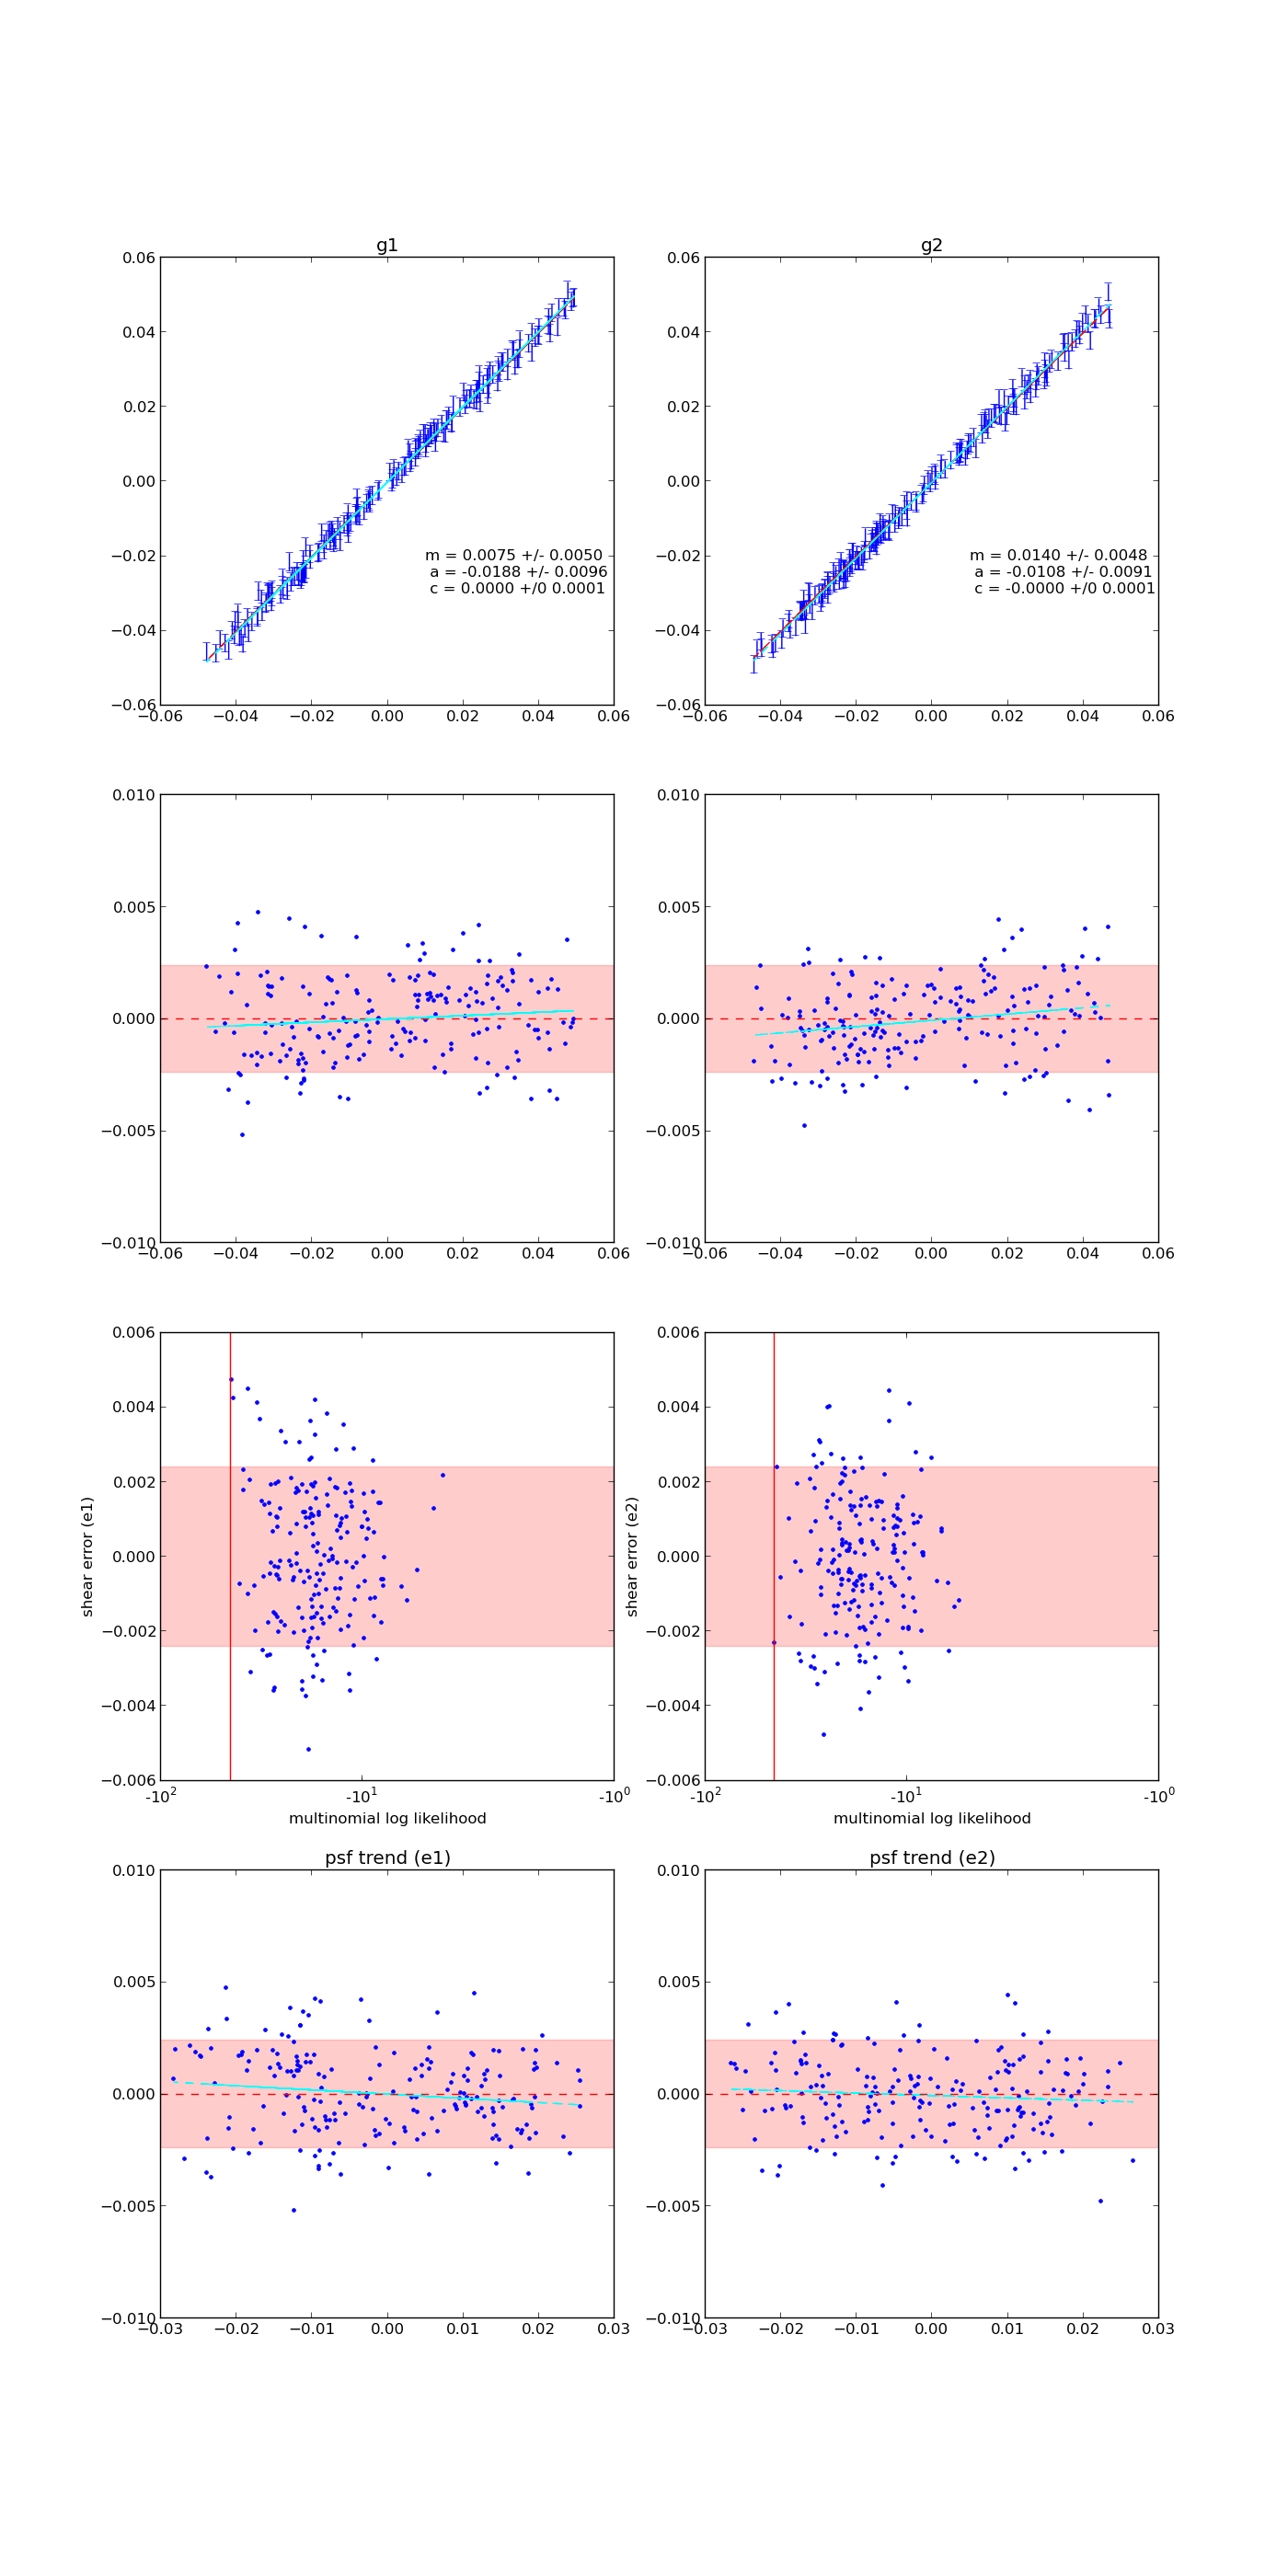
\includegraphics[width=0.31\linewidth]{./Plots/rgc-noaber-regauss-opt-shear_plots.png}
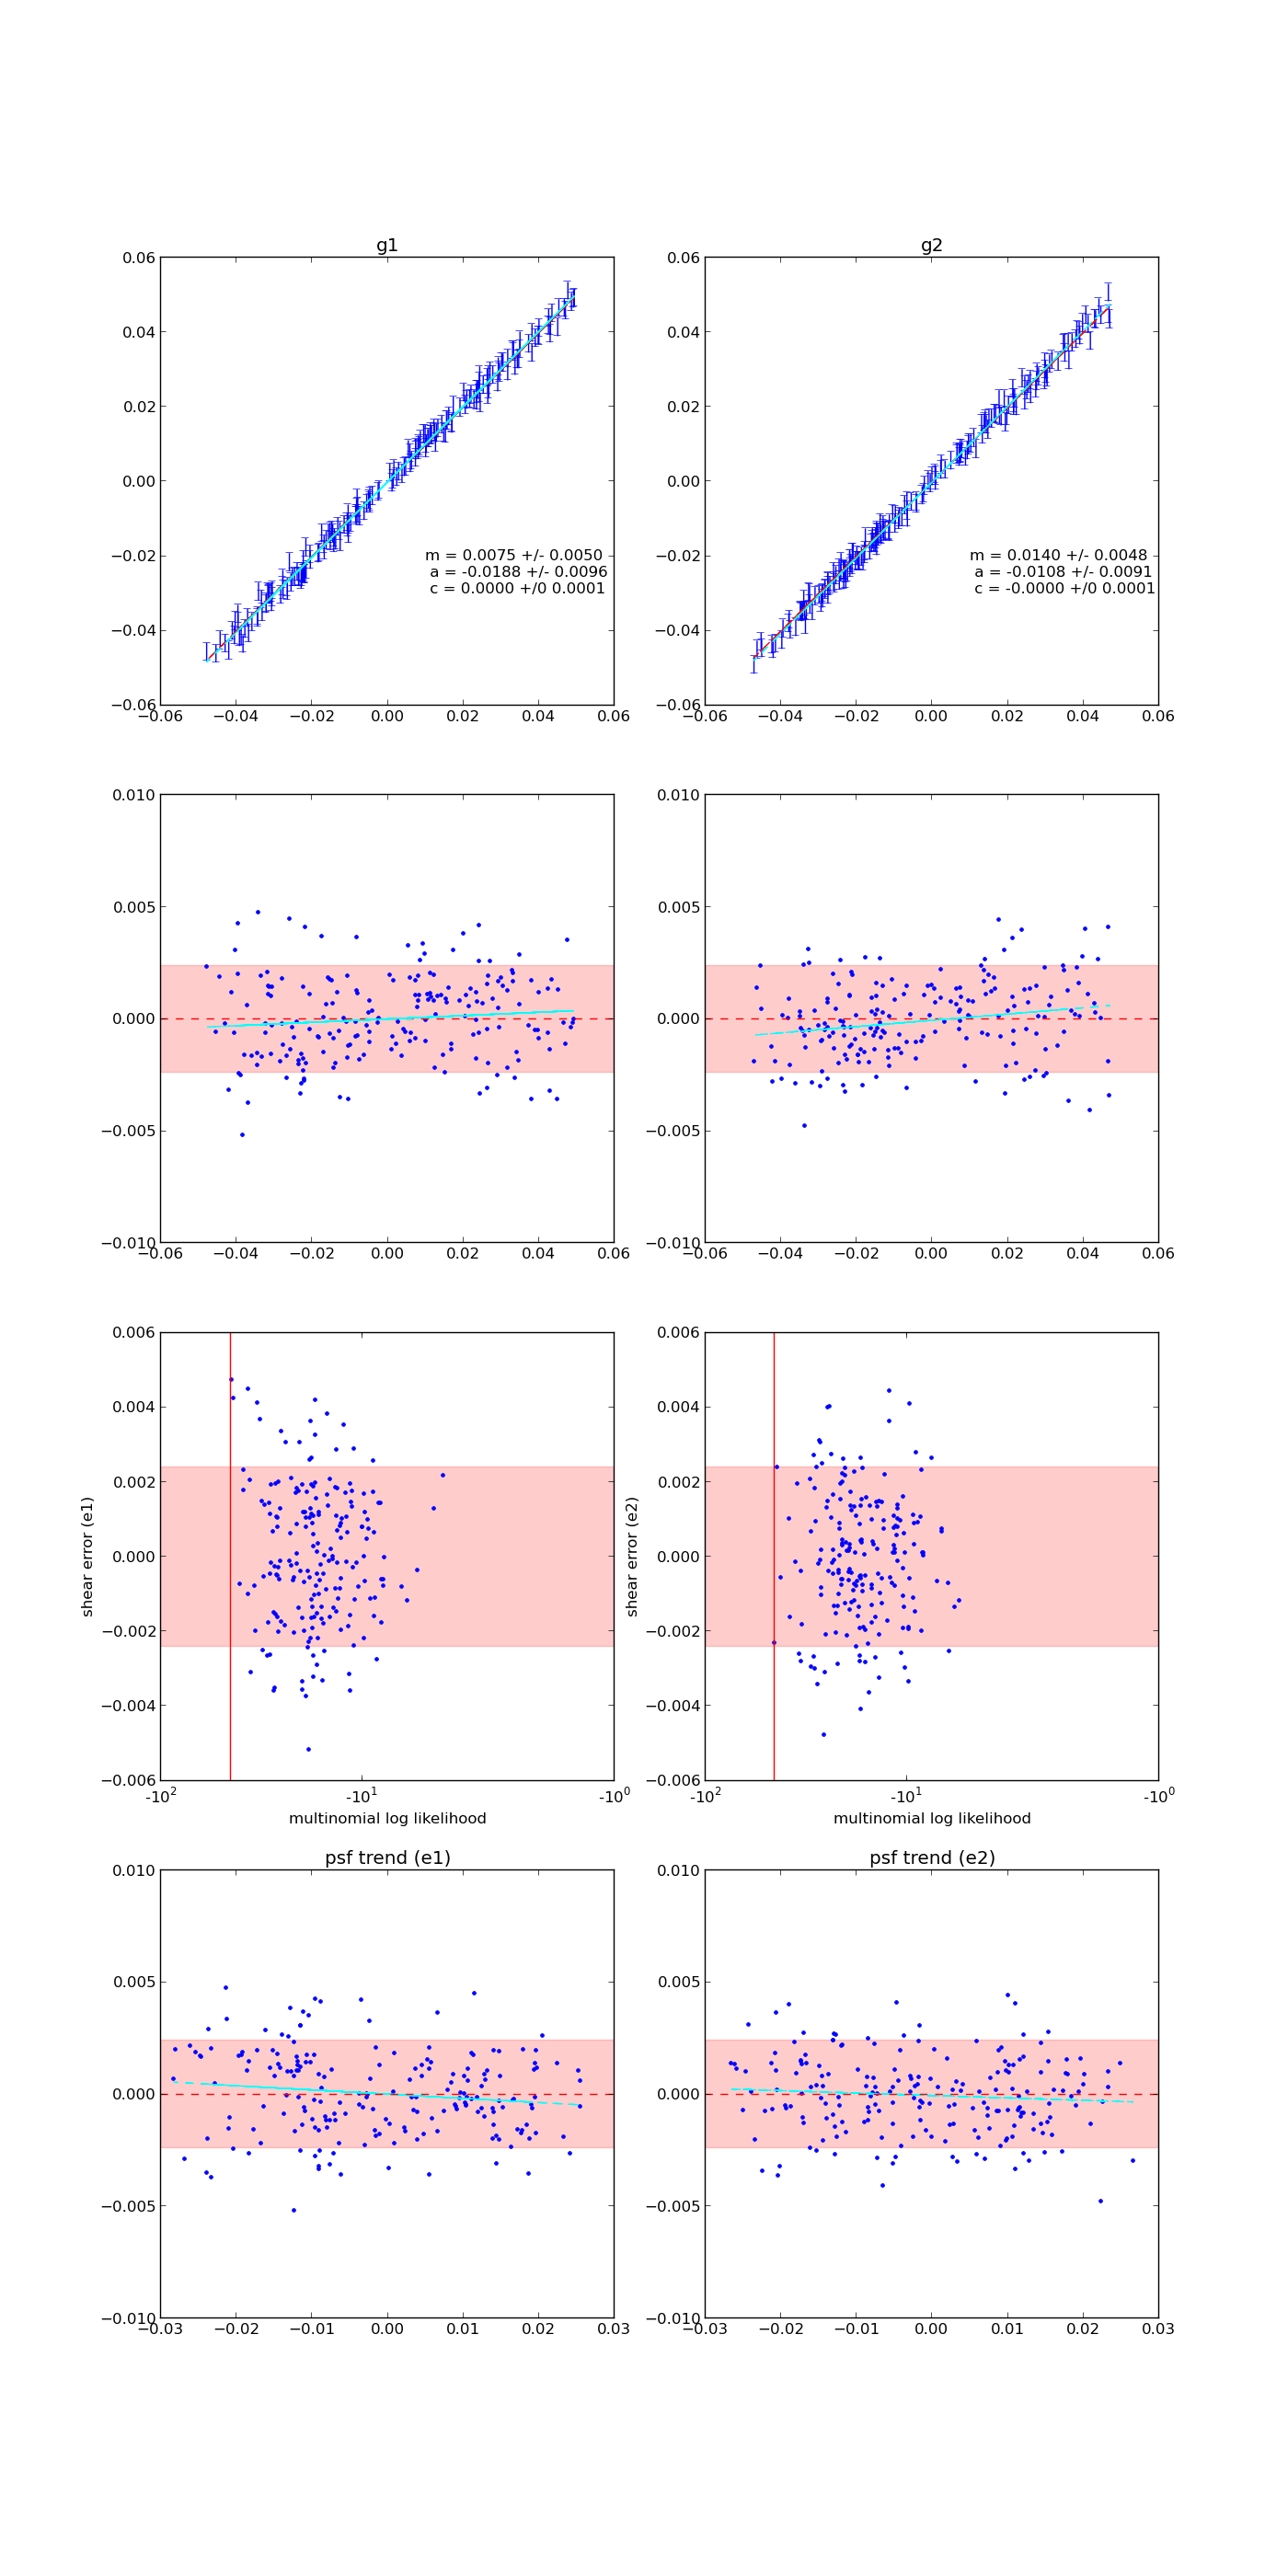
\includegraphics[width=0.31\linewidth]{./Plots/rgc-noaber-regauss-opt-shear_plots.png}
\caption{Results of metacalibration for regauss on RGC with no aberrations. From {\bf right} to {\bf left}: regauss, ksb, moments. Note that we do not have these results for ksb and moments yet.}
\end{figure*}



\begin{figure*}
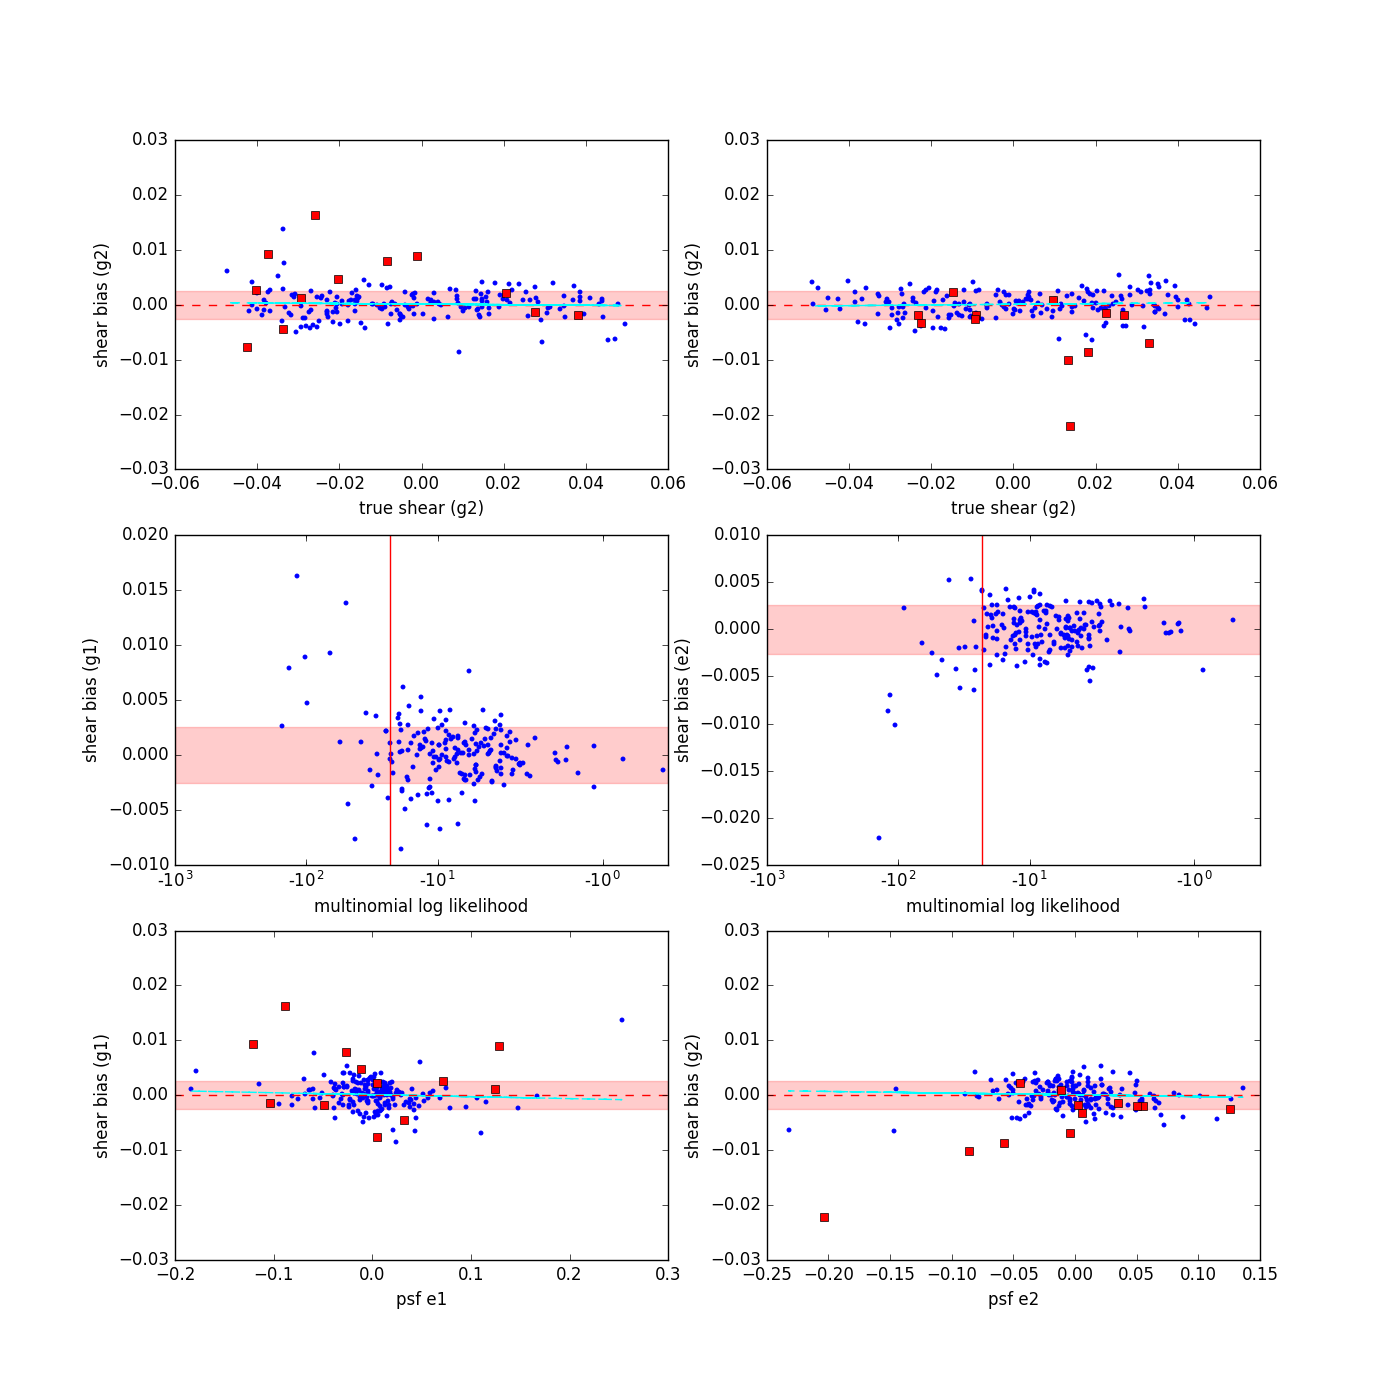
\includegraphics[width=0.31\linewidth]{./Plots/rgc-regauss-opt-shear_plots.png}
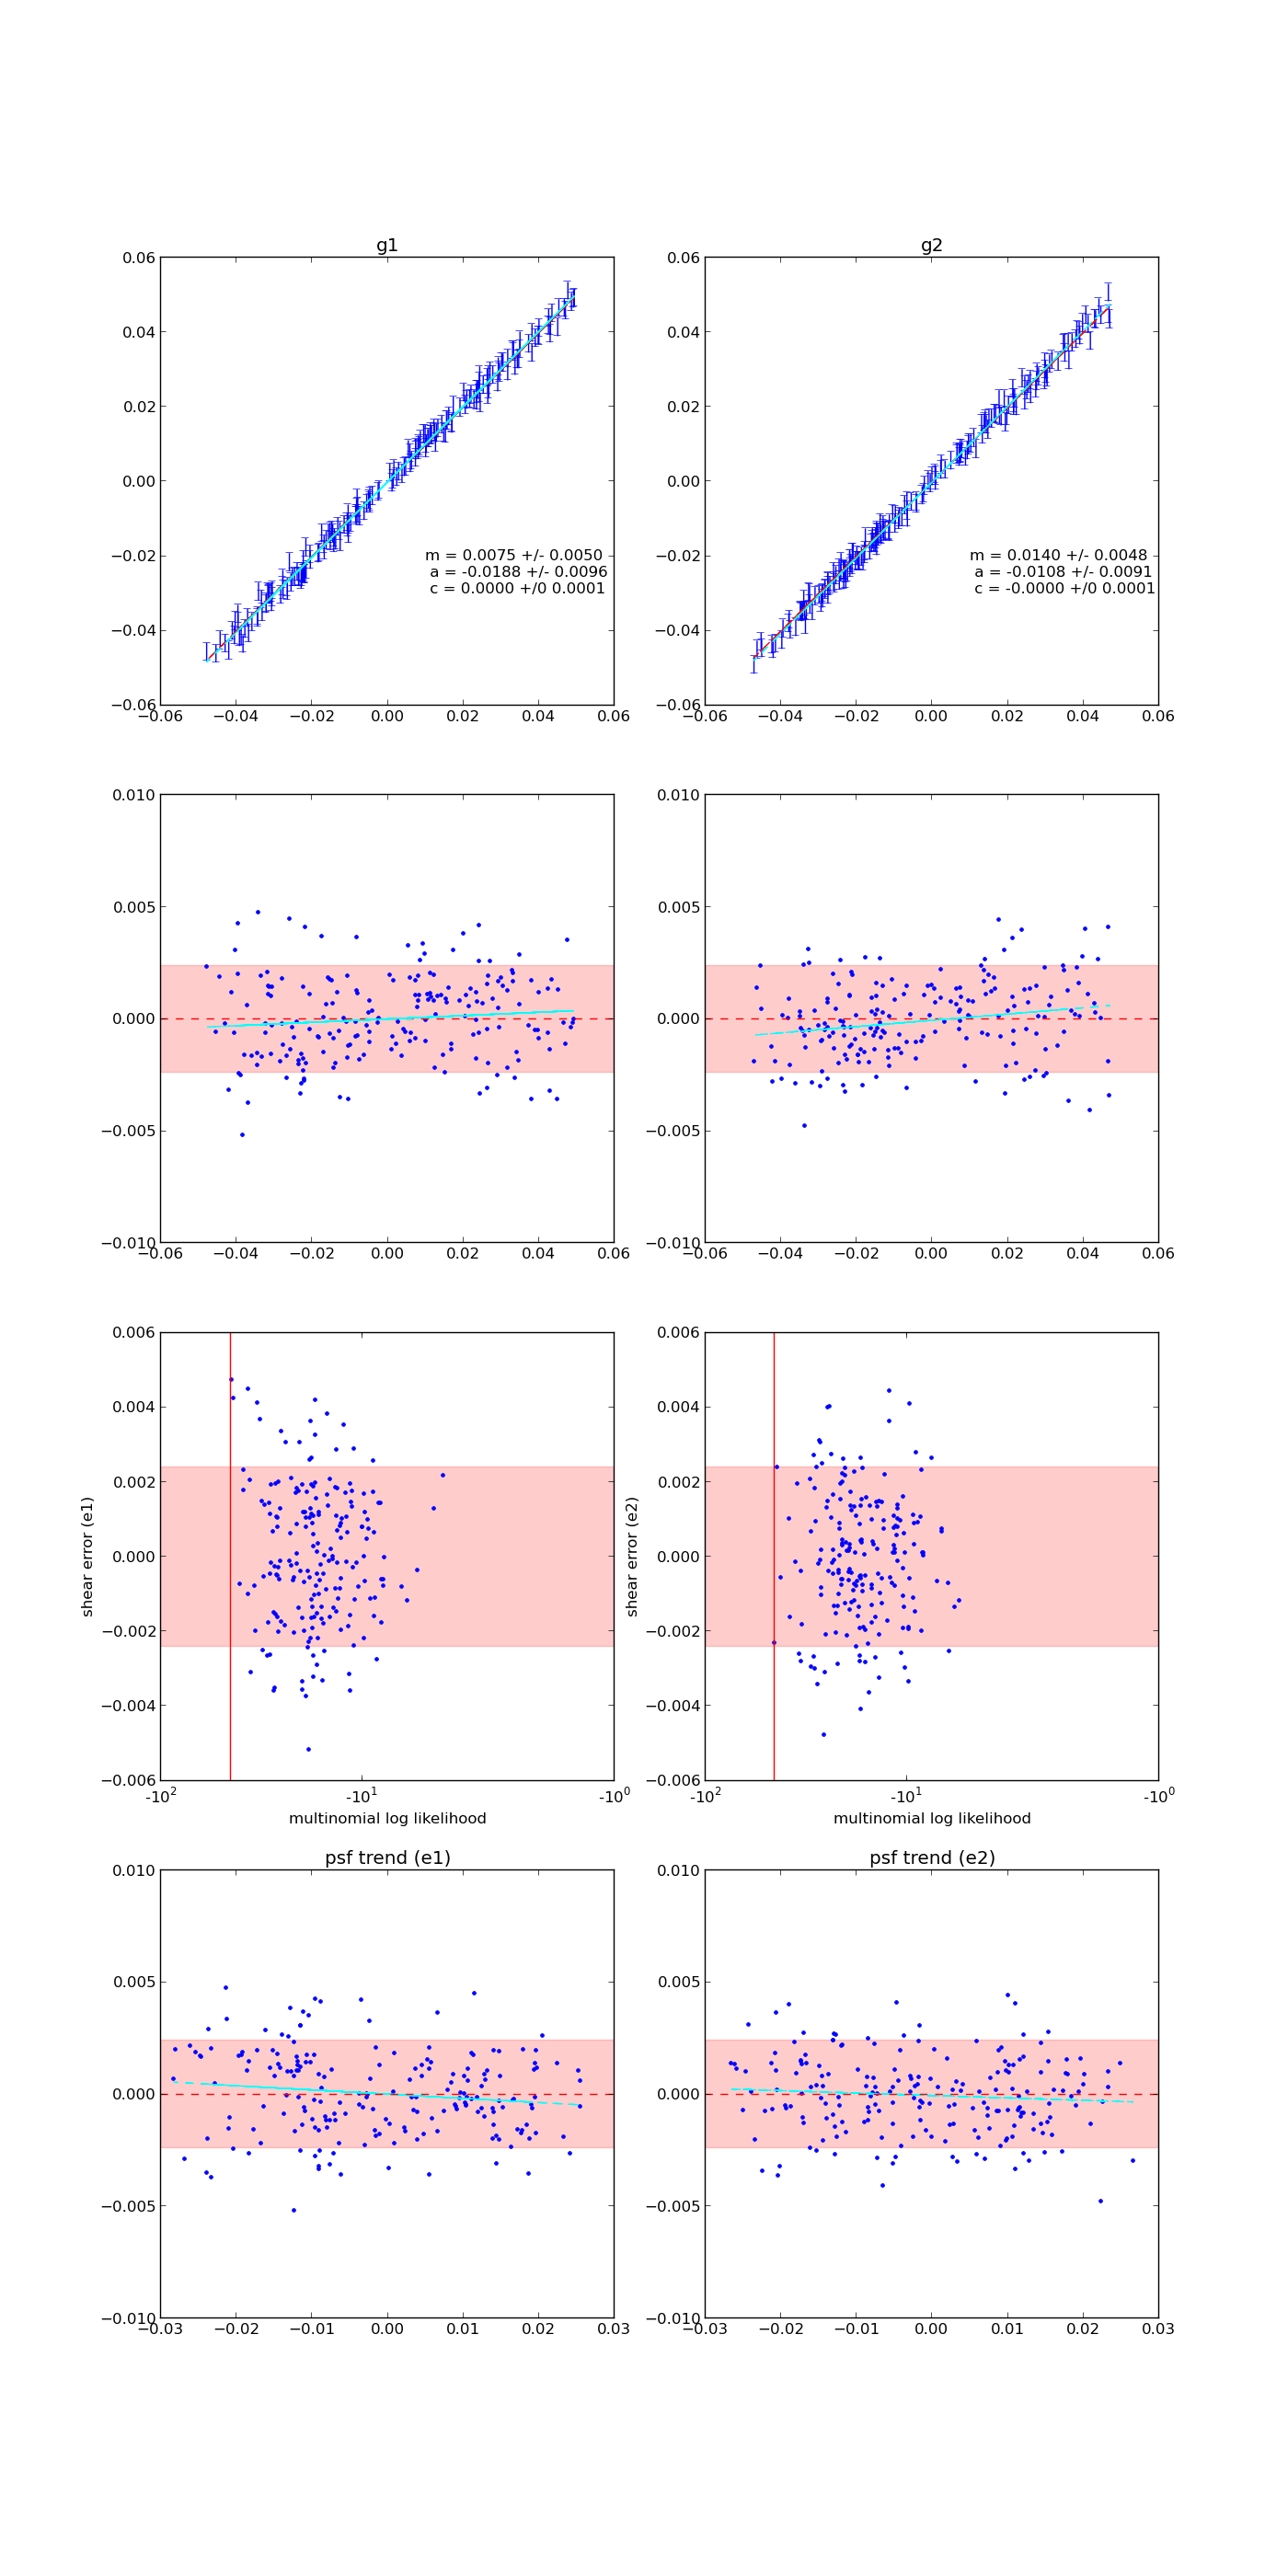
\includegraphics[width=0.31\linewidth]{./Plots/rgc-noaber-regauss-opt-shear_plots.png}
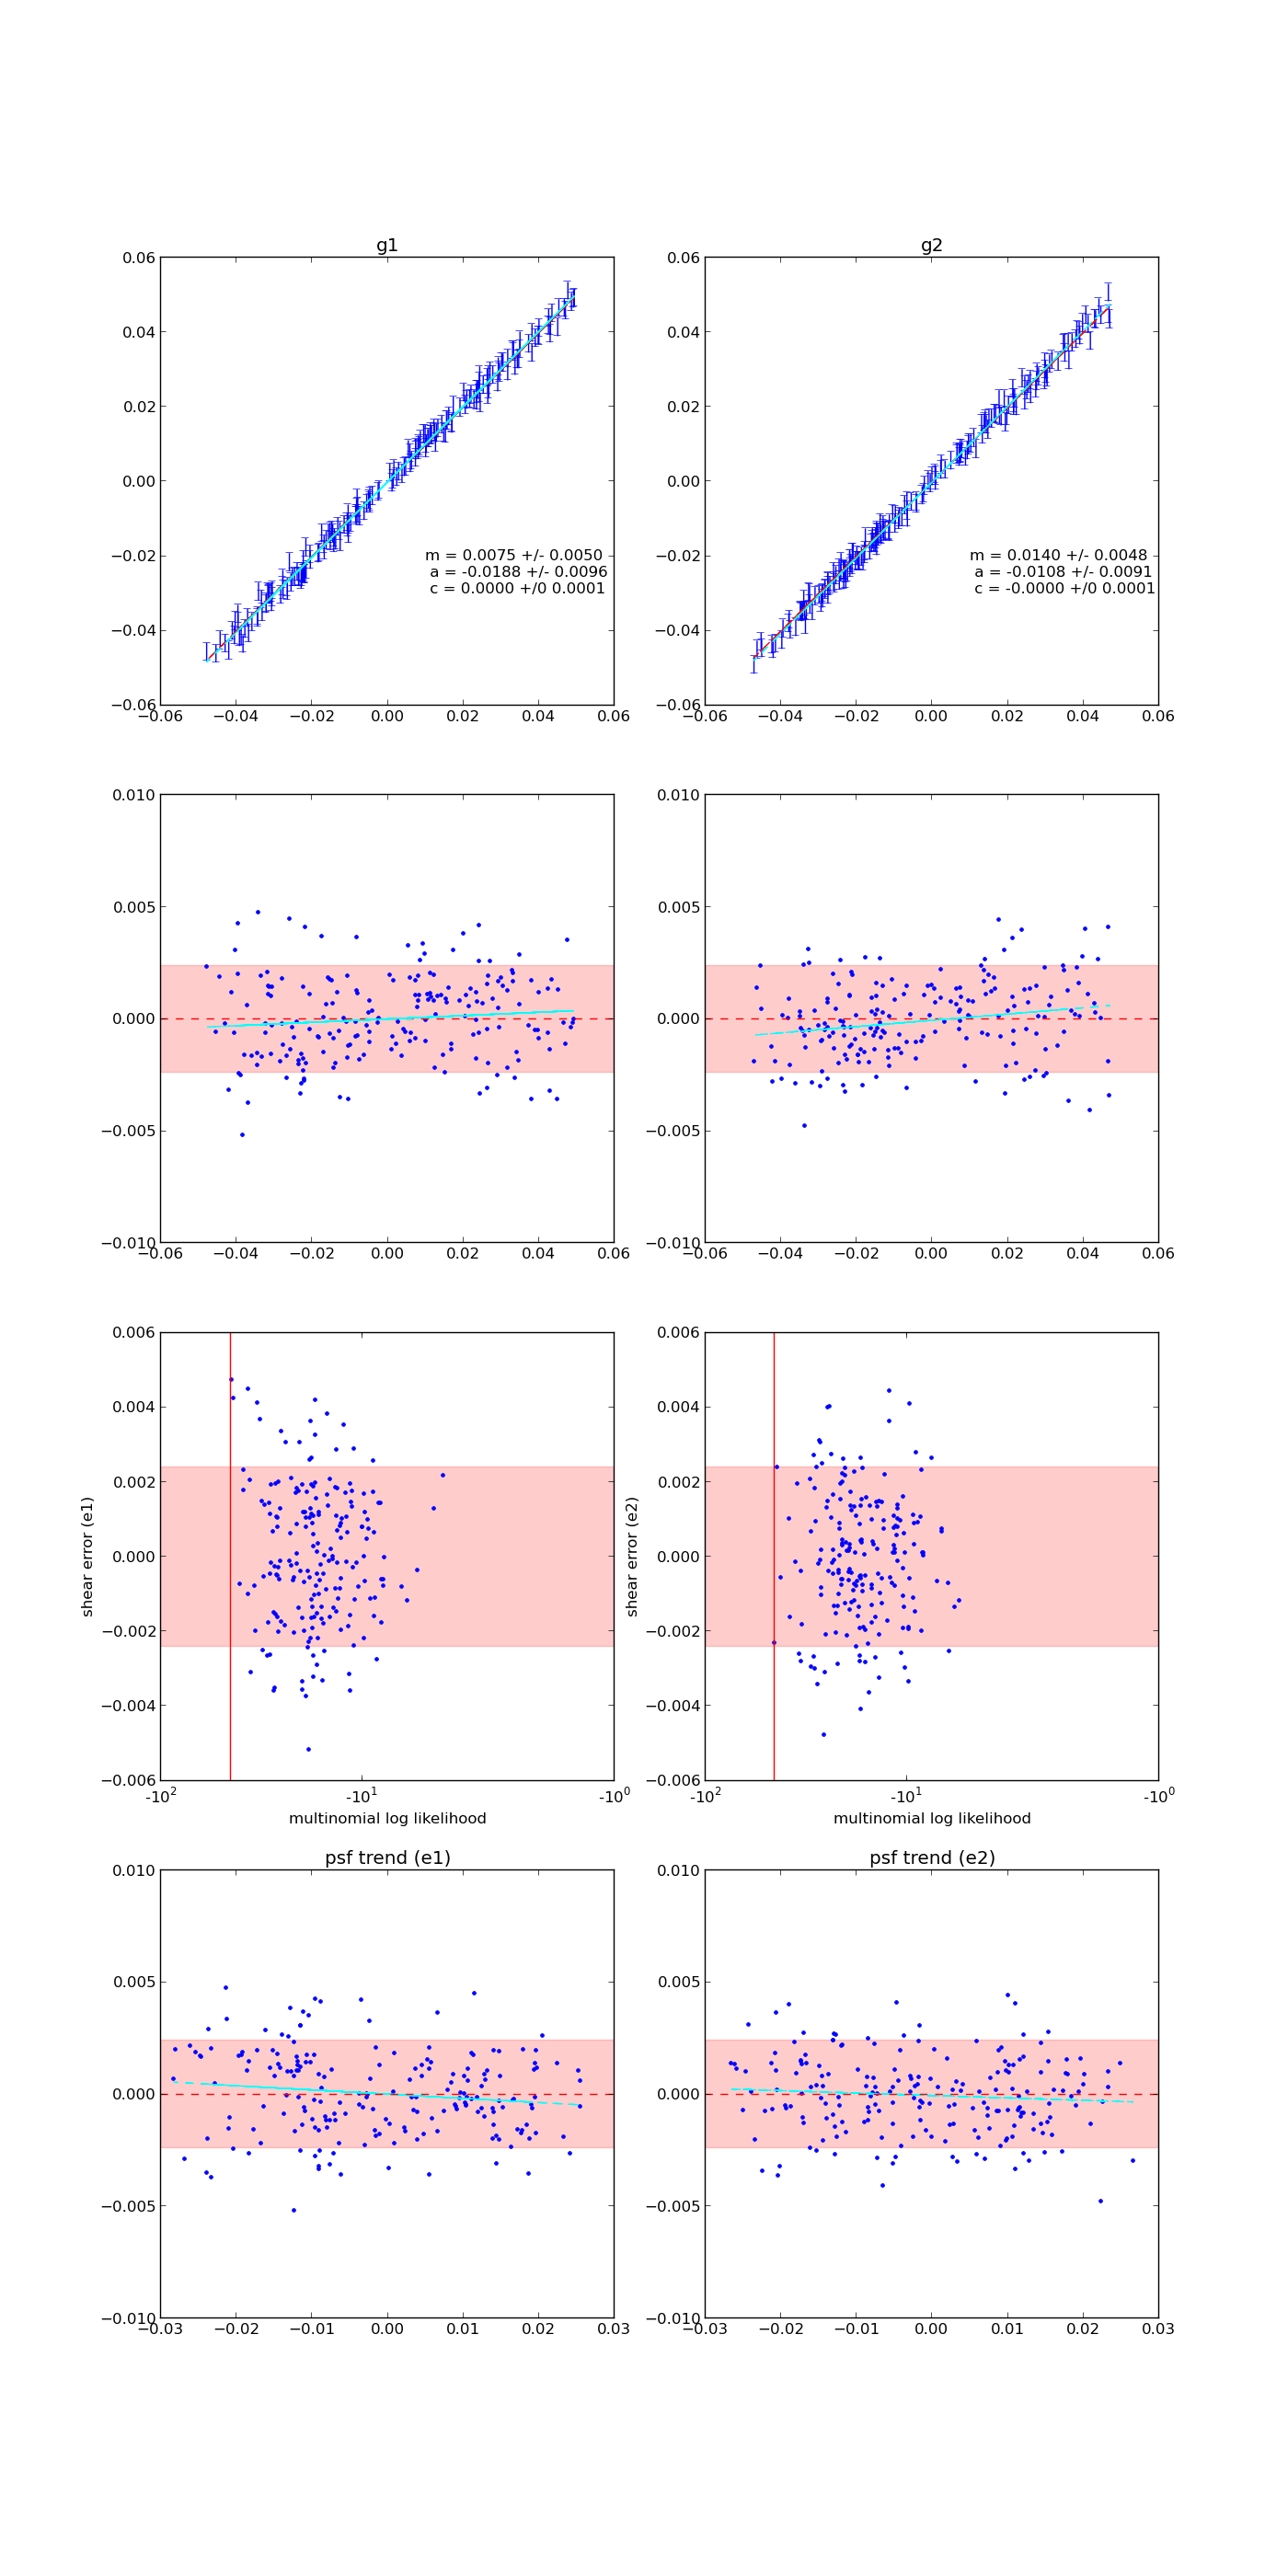
\includegraphics[width=0.31\linewidth]{./Plots/rgc-noaber-regauss-opt-shear_plots.png}
\caption{Results of metacalibration for regauss on RGC with aberrations. From {\bf right} to {\bf left}: regauss, ksb, moments. Note that we do not have these results for ksb and moments yet.}
\end{figure*}


\begin{figure*}
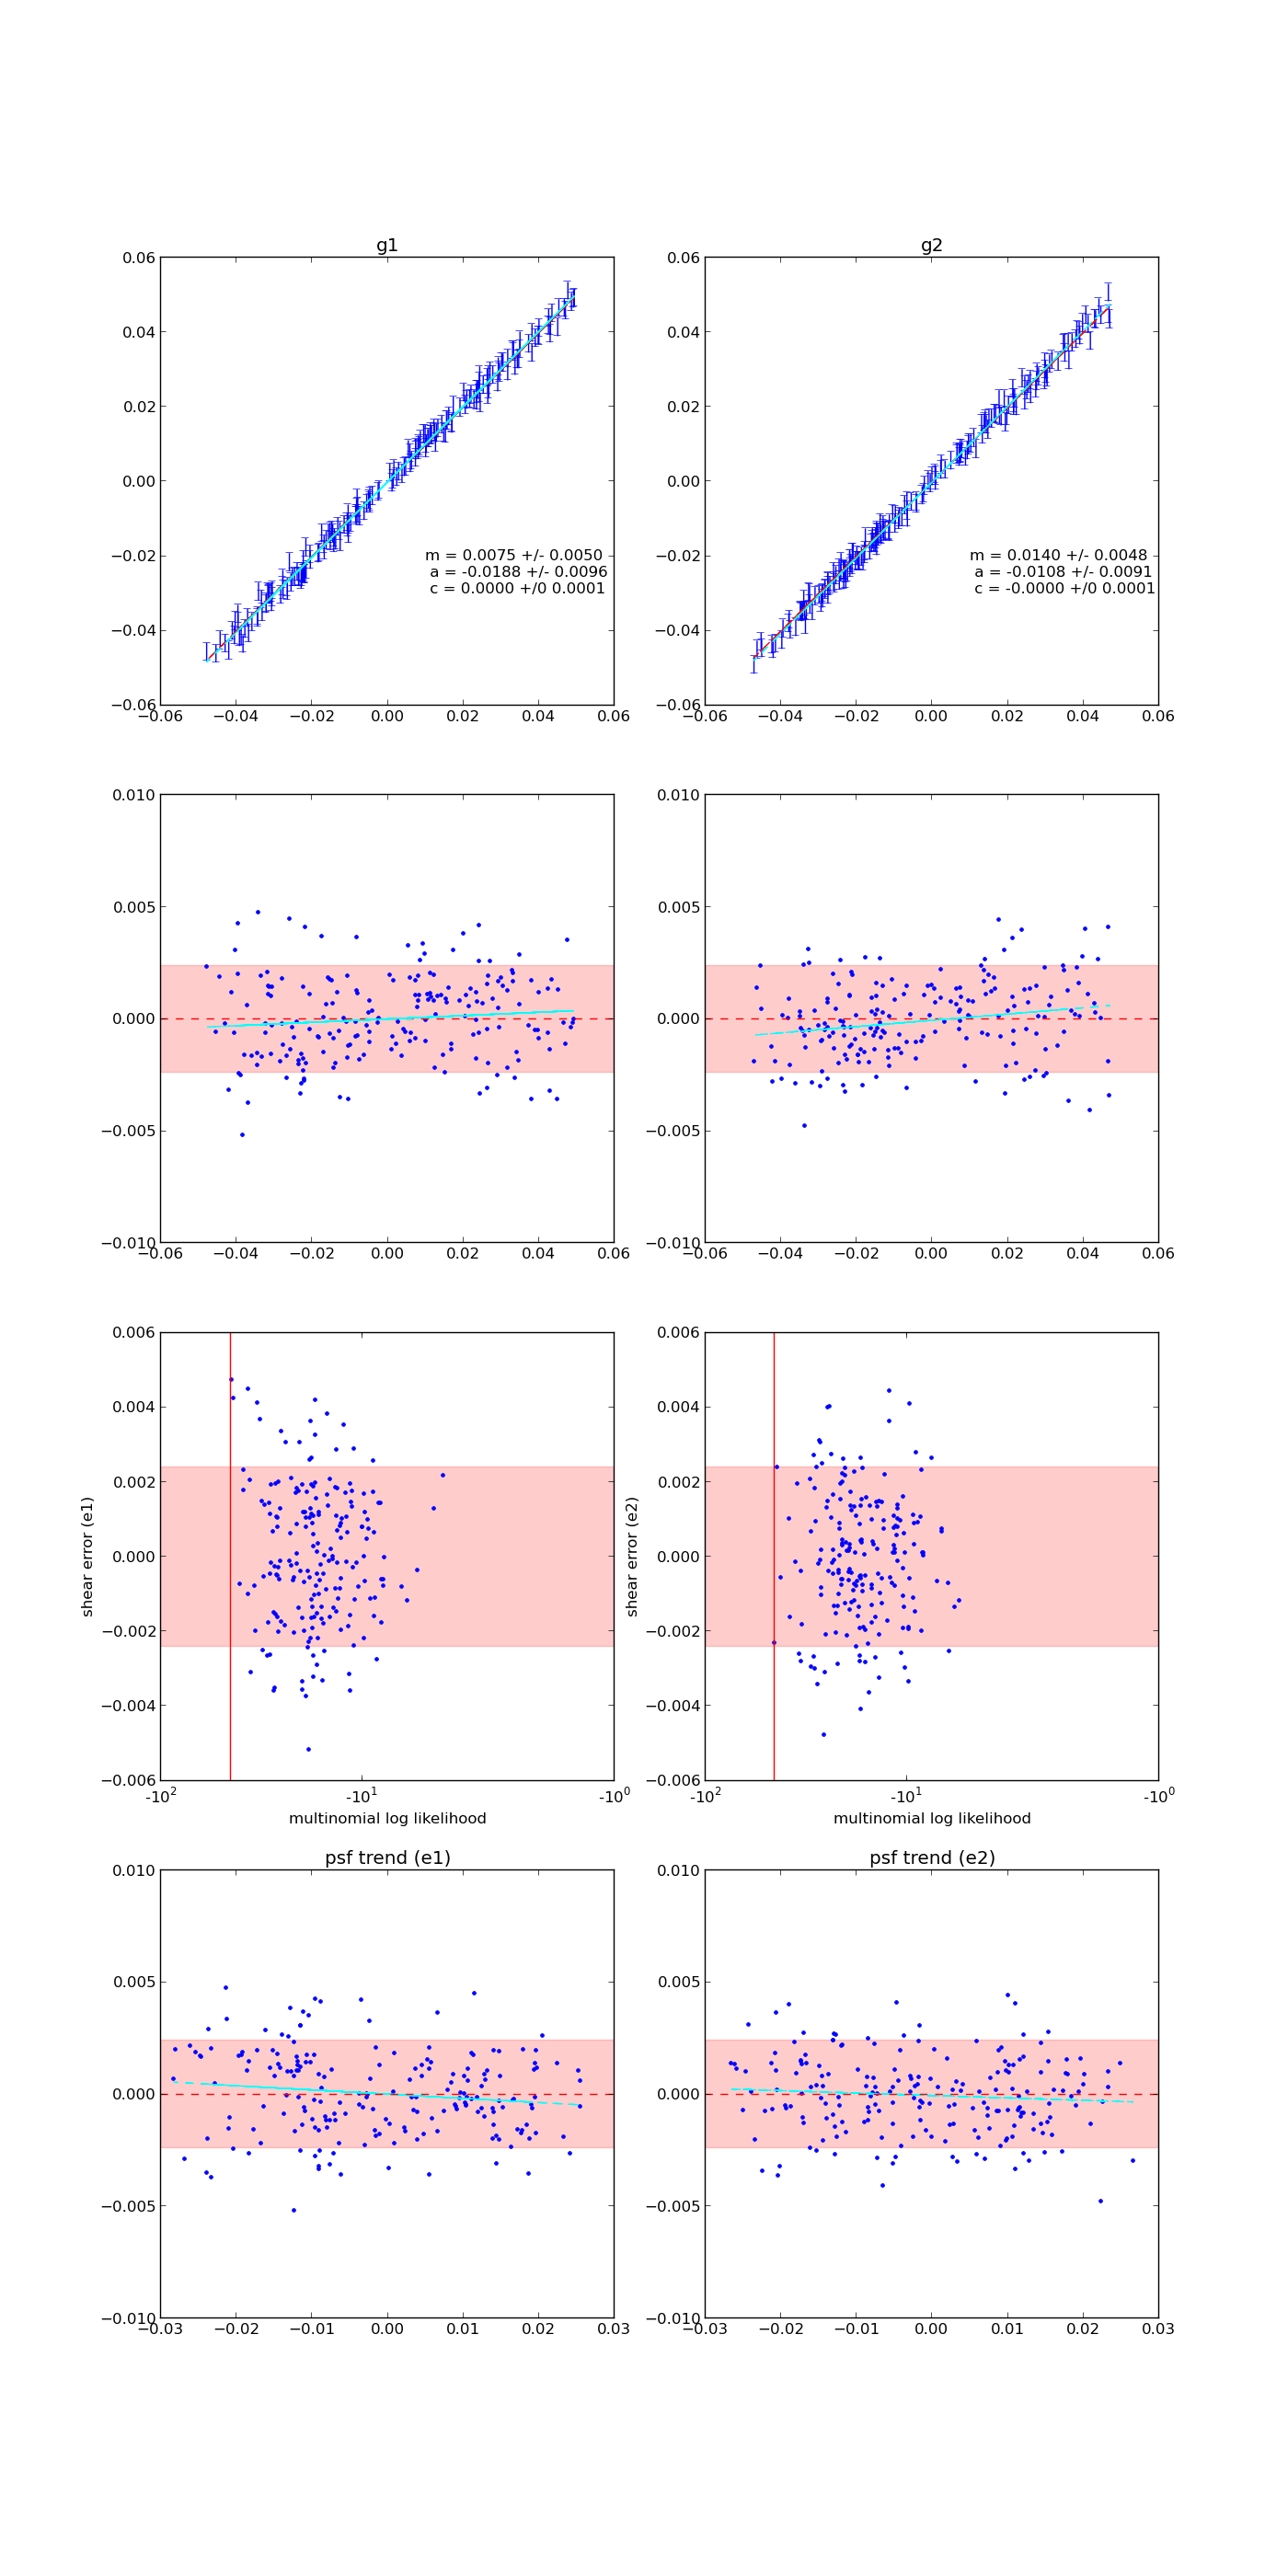
\includegraphics[width=0.3\linewidth]{./Plots/rgc-noaber-regauss-opt-shear_plots.png}
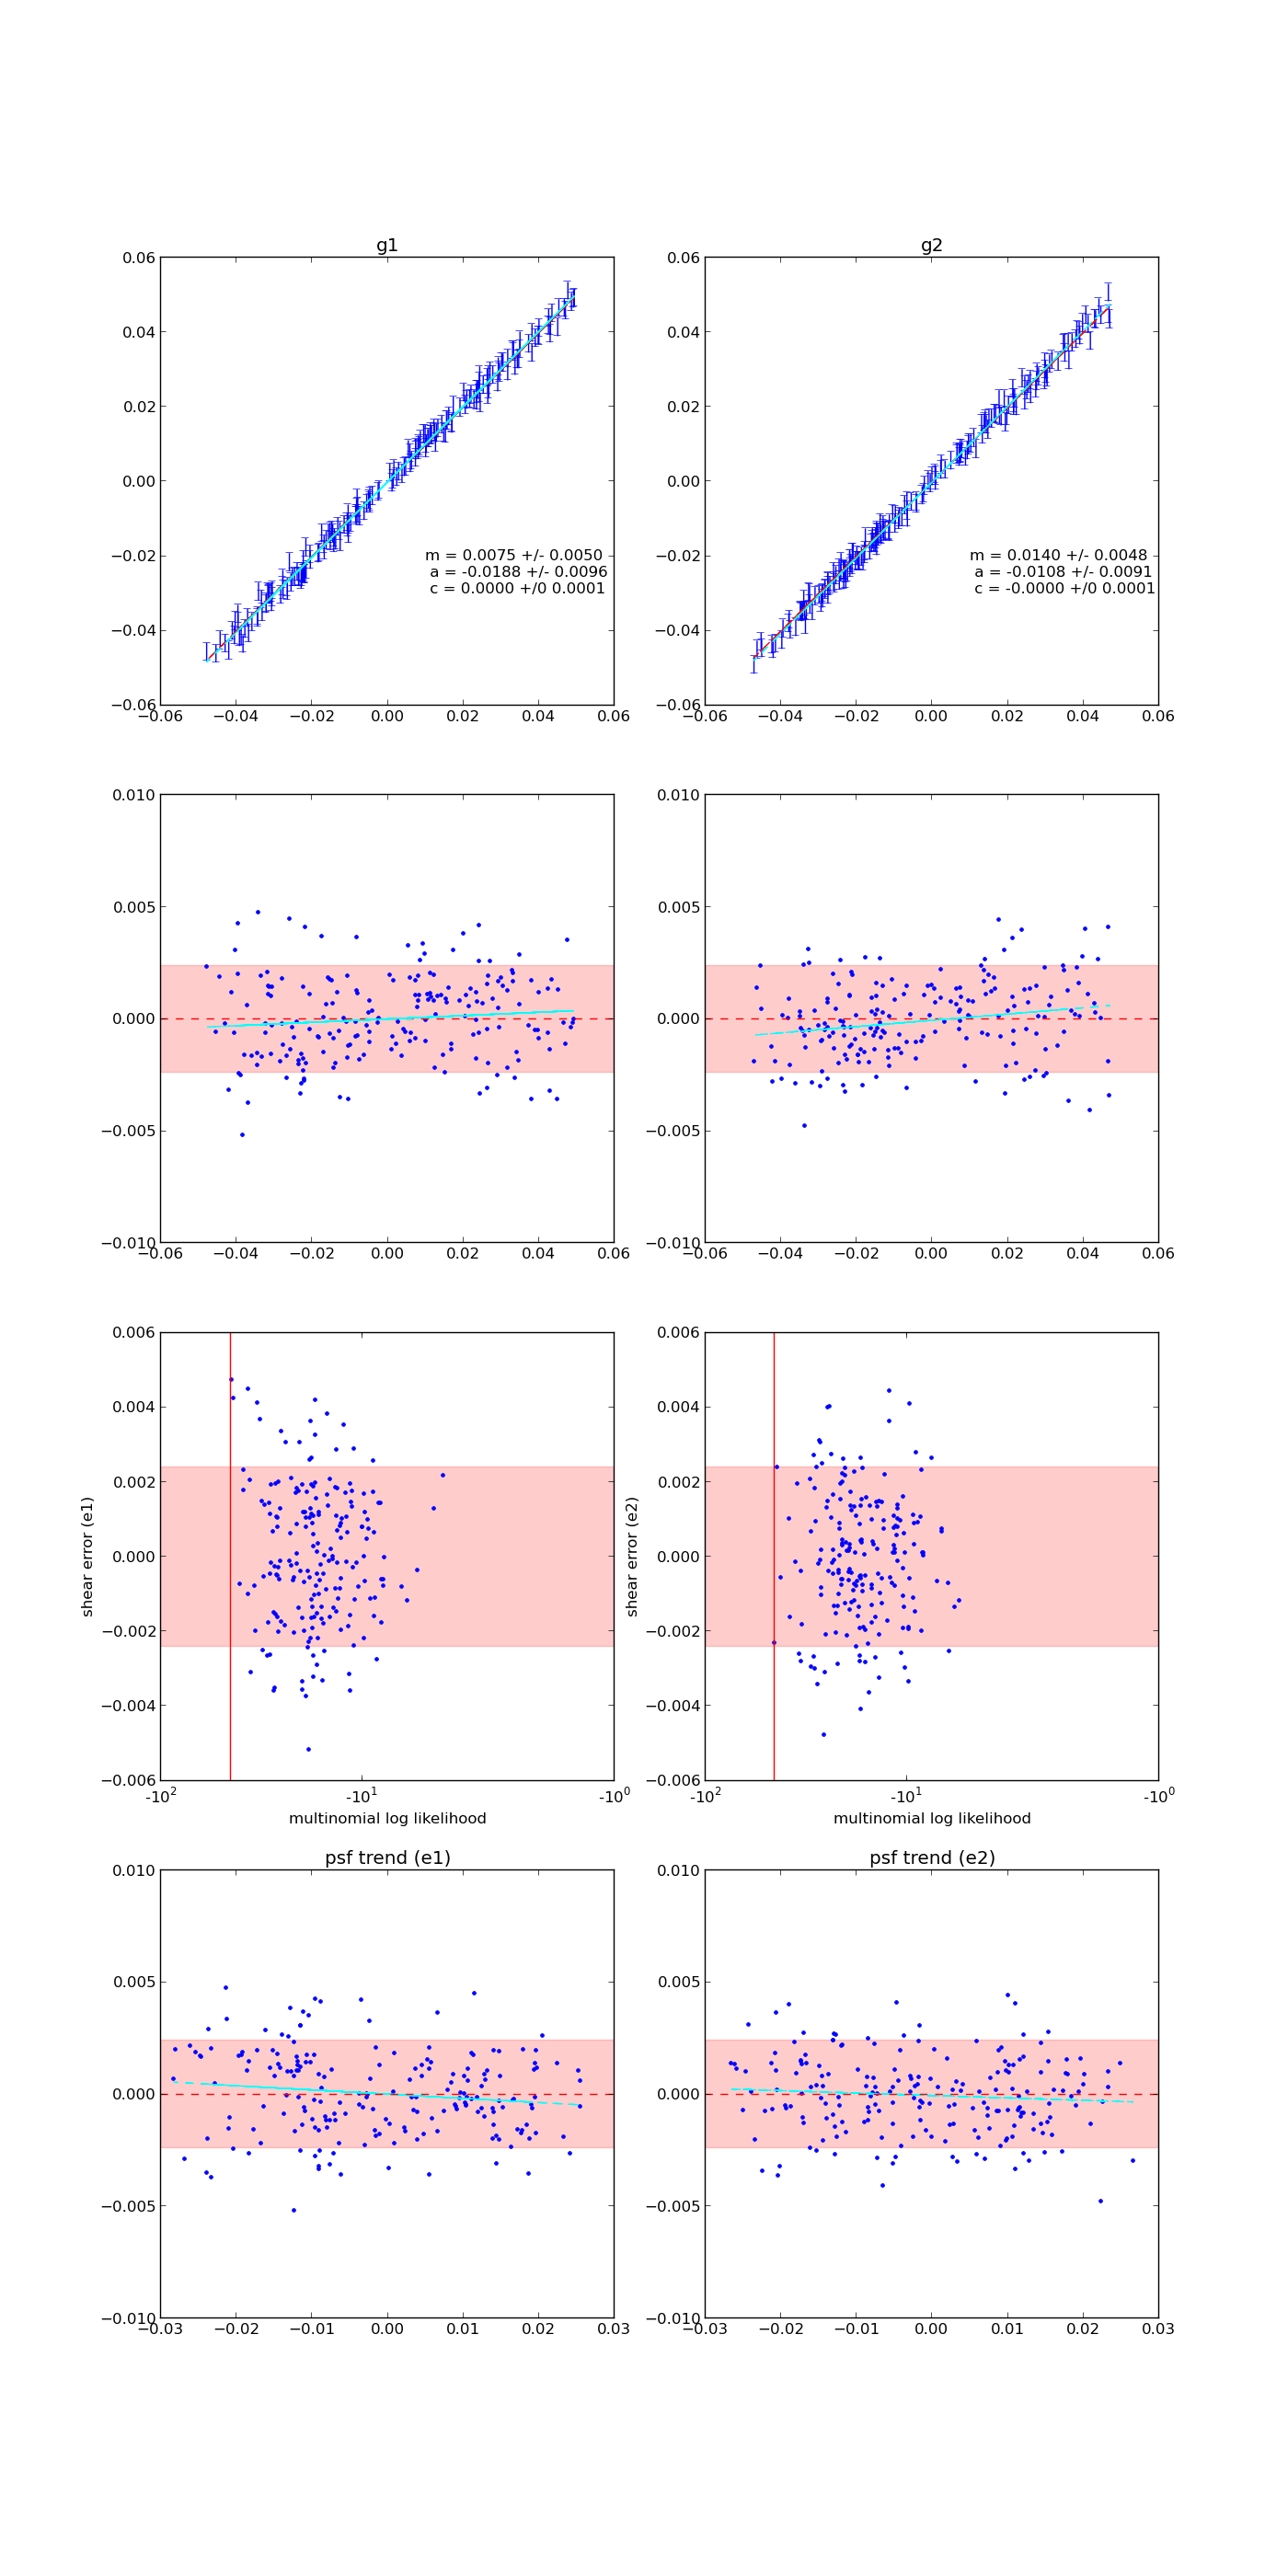
\includegraphics[width=0.3\linewidth]{./Plots/rgc-noaber-regauss-opt-shear_plots.png}
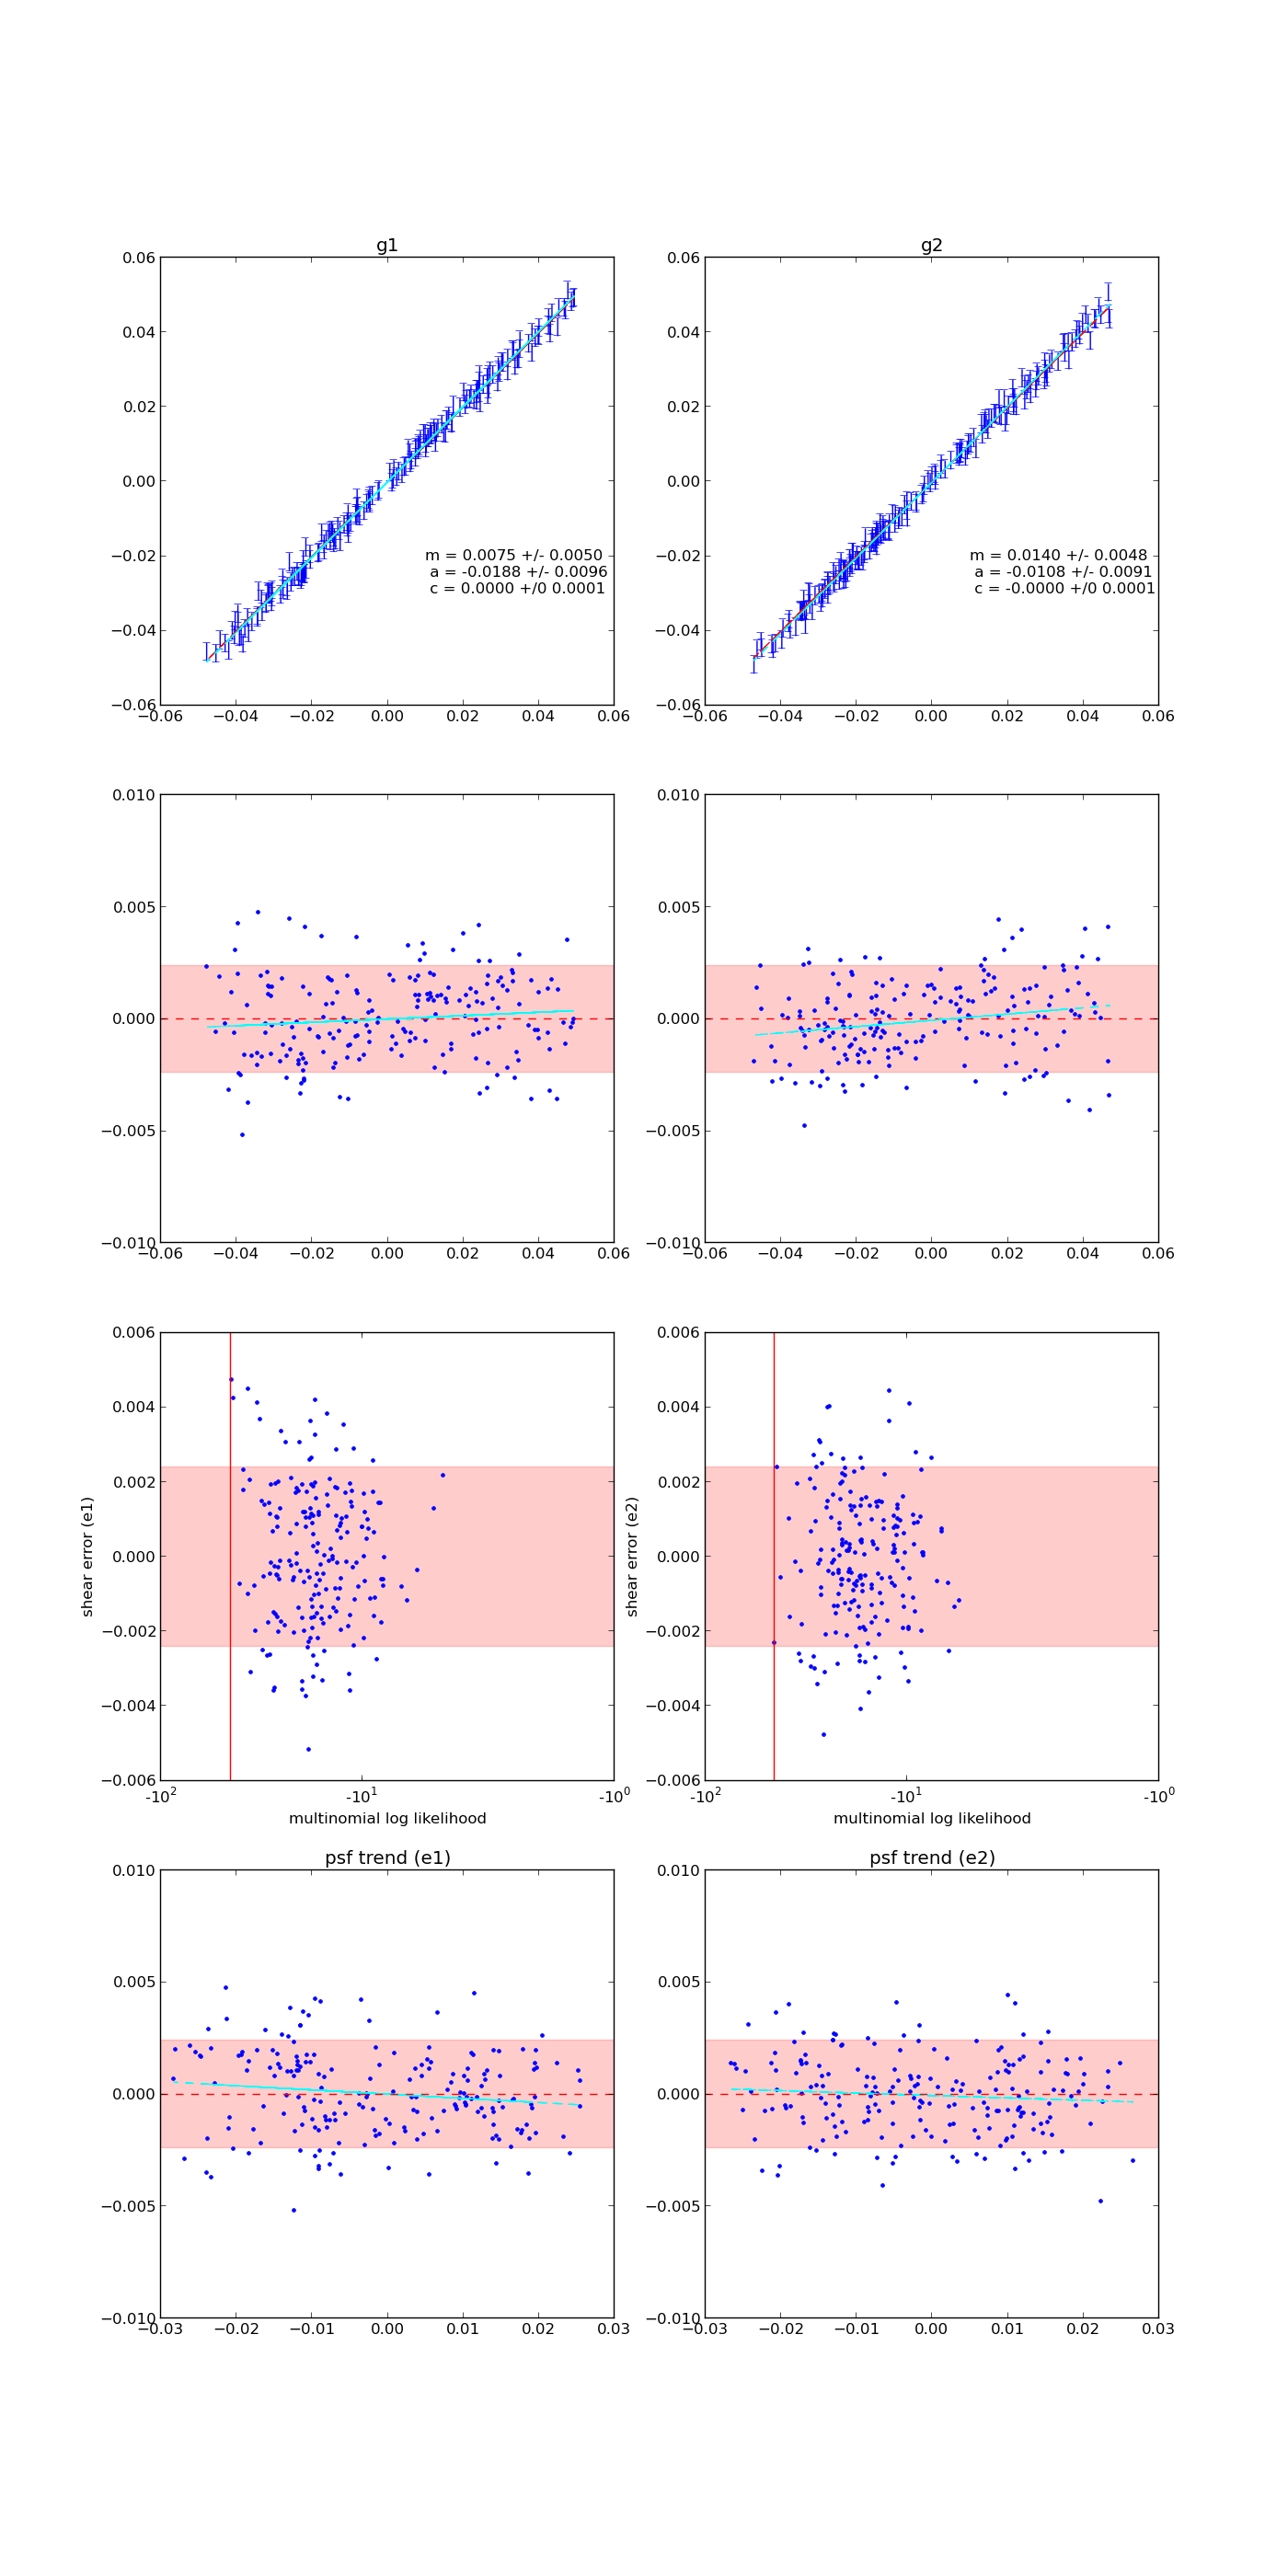
\includegraphics[width=0.3\linewidth]{./Plots/rgc-noaber-regauss-opt-shear_plots.png}
\caption{Results of metacalibration for regauss on RGC with large amplitude but small disperion aberrations. From {\bf right} to {\bf left}: regauss, ksb, moments. Note that we do not have these results for any method yet.}
\end{figure*}

\section{Results}
\towrite{Outline overall results, i.e., {\it veni, vidi, vici}}
\toplotemh{Table of Meta-Calibrated shear and psf calibration biases.}
\toplotrm{Something along the lines of: Great3-style plot showing before/after performance in some projection of m/c/a for regauss/ksb/possibly moments. Something that can easily be compared with one or more figures in the Great3 results paper.}


\section{Applicability to Real Data*}
\towriteemh{Comment on effects that this method may deal with, which we haven’t tested (selection
  biases, other systematics detrending - lack of PSF knowledge?)}
\towriteemh{Comment on what measurements this can be straightforwardly applied to (mass mapping, g-g lensing) and what needs further thought (shear-shear) prior to deployment}
\towriteemh{Comment on effects that this method may or may not play well with -- blending, detector effects, nonlinearity, star-galaxy confusion}
\towriteemh{Comment on noise symmetrization -- we tried this, we don't understand why it didn't work as anticipated, but it doesn't seem to be important at this level of precision.}
\towriteemh{Put computational and implementation difficulty (for a realistic survey pipeline) in
  context. Is this substantially harder than making loads of independent sims? What are the
  prospects for further optimization, or other shortcuts? (silly things like 1-sided derivatives,
  but maybe there are others?)}




\section{Conclusions}
\towrite{Put performance measures from previous sec- tions in context. How do these results compare with the state of the art? Will this be good enough for DES, Kids, LSST?, SuMiRE?}


\bibliographystyle{apj}
\bibliography{bibliography}


\end{document}